\chapter{Hardware Design}
\label{ch:hardware}

This chapter presents the complete microarchitectural design of the \gls{riscv} \gls{vpu}
system. The design implements the \texttt{rv32im\_zicsr\_zve32x\_zvl128b} instruction
set, targeting \gls{asic} tapeout with VLEN~=~128 bits. Every design decision is motivated
by synthesisability, timing closure at the target frequency, and area economy.
The chapter proceeds from the top-level integration, through the scalar pipeline, into
the \gls{vpu} subsystem and its constituent functional units, and concludes with the
memory subsystem and \gls{uart} peripheral.

%% =============================================================================
\section{System Architecture Overview}
\label{sec:system_arch}
%% =============================================================================

\subsection{Top-Level Integration}
\label{subsec:toplevel}

The top-level module \texttt{riscv\_vpu\_top\_v4} integrates five major subsystems on a
common clock domain: the five-stage scalar pipeline (\texttt{pipelined\_vpu}), the
\gls{vpu} subsystem (\texttt{vproc\_system\_wrapper}), a synchronous dual-port data
memory (\texttt{dmem\_sync}), a synchronous instruction memory (\texttt{imem\_sync}),
and a \gls{uart} controller. The module is parameterised by \texttt{CLK\_FREQ} and
\texttt{BAUD\_RATE} so that simulations may run at a high baud divisor without modifying
firmware; the default configuration uses $\mathit{CLK\_FREQ} = 14{,}745{,}600$~Hz and
$\mathit{BAUD\_RATE} = 115{,}200$~baud, yielding a divisor of 128.

\begin{figure}[H]
  \centering
  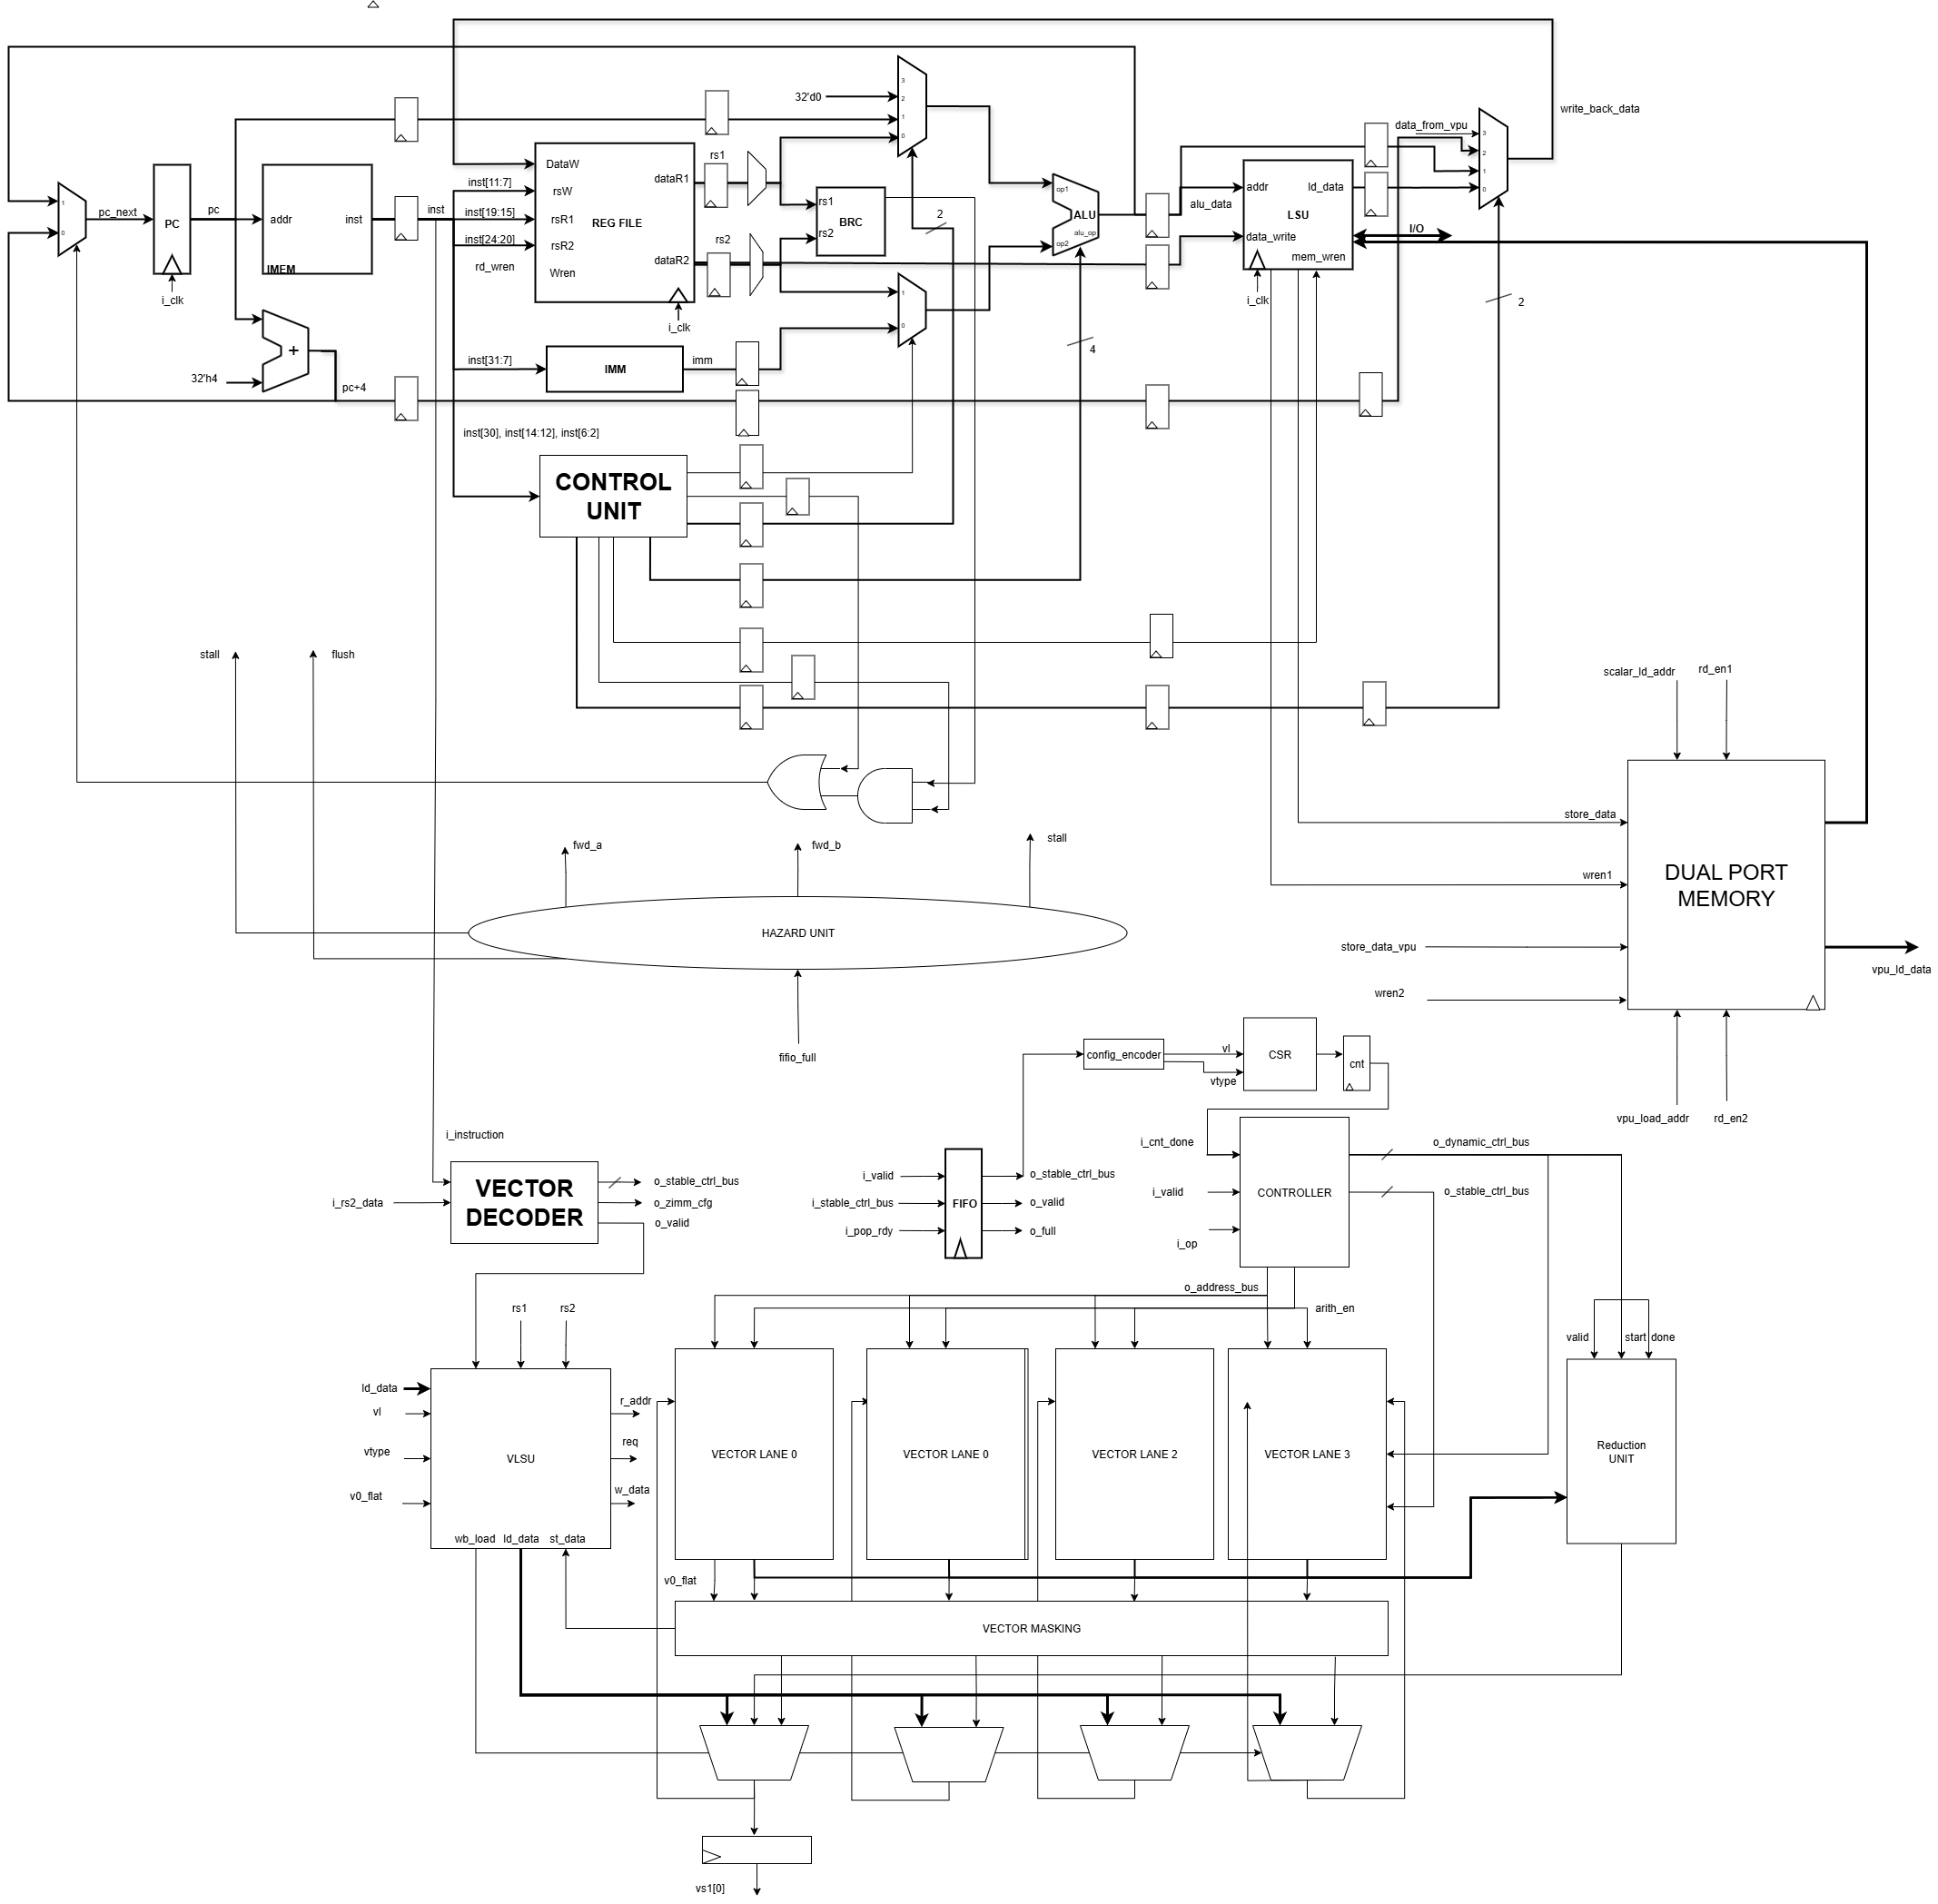
\includegraphics[width=\textwidth]{../image/TOP_design.png}
  \caption{Top-level block diagram of \texttt{riscv\_vpu\_top}: scalar pipeline,
           VPU subsystem, IMEM, DMEM (dual-port), and interconnect buses.}
  \label{fig:top_design}
\end{figure}

Address decoding is performed inline without a bus arbiter. The scalar core presents
a 32-bit byte address on its DMEM port. A single combinational comparator checks
whether bits~[31:8] equal \texttt{0xFF0000}; if so, the transaction is steered to the
\gls{uart} TL-UL interface; otherwise it reaches \texttt{dmem\_sync} port~A. This
approach keeps the critical path short and eliminates the area overhead of a full
interconnect fabric, which is appropriate for a single-master system.

\subsection{Clock and Reset Distribution}
\label{subsec:clk_reset}

A single clock, \texttt{i\_clk}, is used throughout the design. The external reset pin
\texttt{i\_reset} is active-high for compatibility with FPGA push-button convention;
it is immediately inverted to \texttt{rst\_n} (active-low) at the top level so that
every submodule sees the \gls{asic}-standard active-low synchronous reset interface.
All flip-flops in \texttt{vproc\_system\_wrapper} and \texttt{vproc\_vec\_lsu} use
\texttt{posedge clk / negedge rst\_n}, producing synthesisable reset trees. The scalar
pipeline registers use synchronous active-high reset (\texttt{i\_reset}) directly,
following the convention established in the \gls{riscv} scalar core.

No clock gating cells are instantiated explicitly in RTL; clock enable signals
(\texttt{write\_en[3:0]} on the \gls{vrf}, pipeline stall enables, and VLSU advance
conditions) are present on every register bank to allow automatic clock-gating
inference by a downstream synthesis tool. The power-reduction benefit is most
significant on the \gls{vrf} banks, which collectively hold $32 \times 4 \times
8 = 1024$ flip-flops, and would otherwise toggle unnecessarily on every cycle.

\subsection{Signal Interface Summary}
\label{subsec:sig_table}

\begin{table}[H]
\centering
\caption{Top-level inter-subsystem buses and their widths}
\label{tab:top_buses}
\begin{tabular}{llcl}
\toprule
\textbf{Bus / Signal Group} & \textbf{Direction} & \textbf{Width (bits)} & \textbf{Description} \\
\midrule
\texttt{PC} (scalar $\to$ IMEM)               & Scalar $\to$ IMEM   & 32  & Word-aligned program counter \\
\texttt{instr} (IMEM $\to$ scalar)            & IMEM $\to$ Scalar   & 32  & Registered instruction word \\
Scalar DMEM port A (addr/wdata/rdata/we/be/re) & Scalar $\leftrightarrow$ DMEM & 32+32+32+1+4+1 & Scalar load/store \\
VLSU DMEM port B (addr/wdata/rdata/req/we/be/ready) & VPU $\leftrightarrow$ DMEM & 32+32+32+1+1+4+1 & Vector load/store \\
\texttt{vpu\_insn\_vld}                        & Scalar $\to$ VPU    & 1   & OP-V instruction valid \\
\texttt{vpu\_insn}                             & Scalar $\to$ VPU    & 32  & Dispatched instruction \\
\texttt{vpu\_rs1\_data}, \texttt{vpu\_rs2\_data} & Scalar $\to$ VPU  & 32  & Scalar register operands \\
\texttt{vpu\_ready}                            & VPU $\to$ Scalar    & 1   & Back-pressure: 0 = stall scalar \\
\texttt{vpu\_cfg\_done}                        & VPU $\to$ Scalar    & 1   & \texttt{vsetvl*} commit pulse \\
\texttt{vpu\_vl\_remain}                       & VPU $\to$ Scalar    & 32  & New \texttt{vl} for scalar \texttt{rd} writeback \\
TL-UL A channel (\texttt{uart\_tl\_a})         & Scalar $\to$ UART   & 71  & TL-UL A-channel bundle \\
TL-UL D channel (\texttt{uart\_tl\_d})         & UART $\to$ Scalar   & 33  & TL-UL D-channel bundle \\
\texttt{uart\_rx}, \texttt{uart\_tx}            & External I/O        & 1 each & Serial data lines \\
\bottomrule
\end{tabular}
\end{table}

%% =============================================================================
\section{Scalar RISC-V Core}
\label{sec:scalar_core}
%% =============================================================================

The scalar core implements the \texttt{rv32im\_zicsr} subset as a classical five-stage
in-order pipeline: Instruction Fetch (IF), Instruction Decode (ID), Execute (EX),
Memory (MEM), and Write-Back (WB). The design is contained in the
\texttt{pipelined\_vpu} module and uses synchronous active-high reset internally.

\subsection{Pipeline Structure}
\label{subsec:pipeline_structure}

\begin{figure}[H]
  \centering
  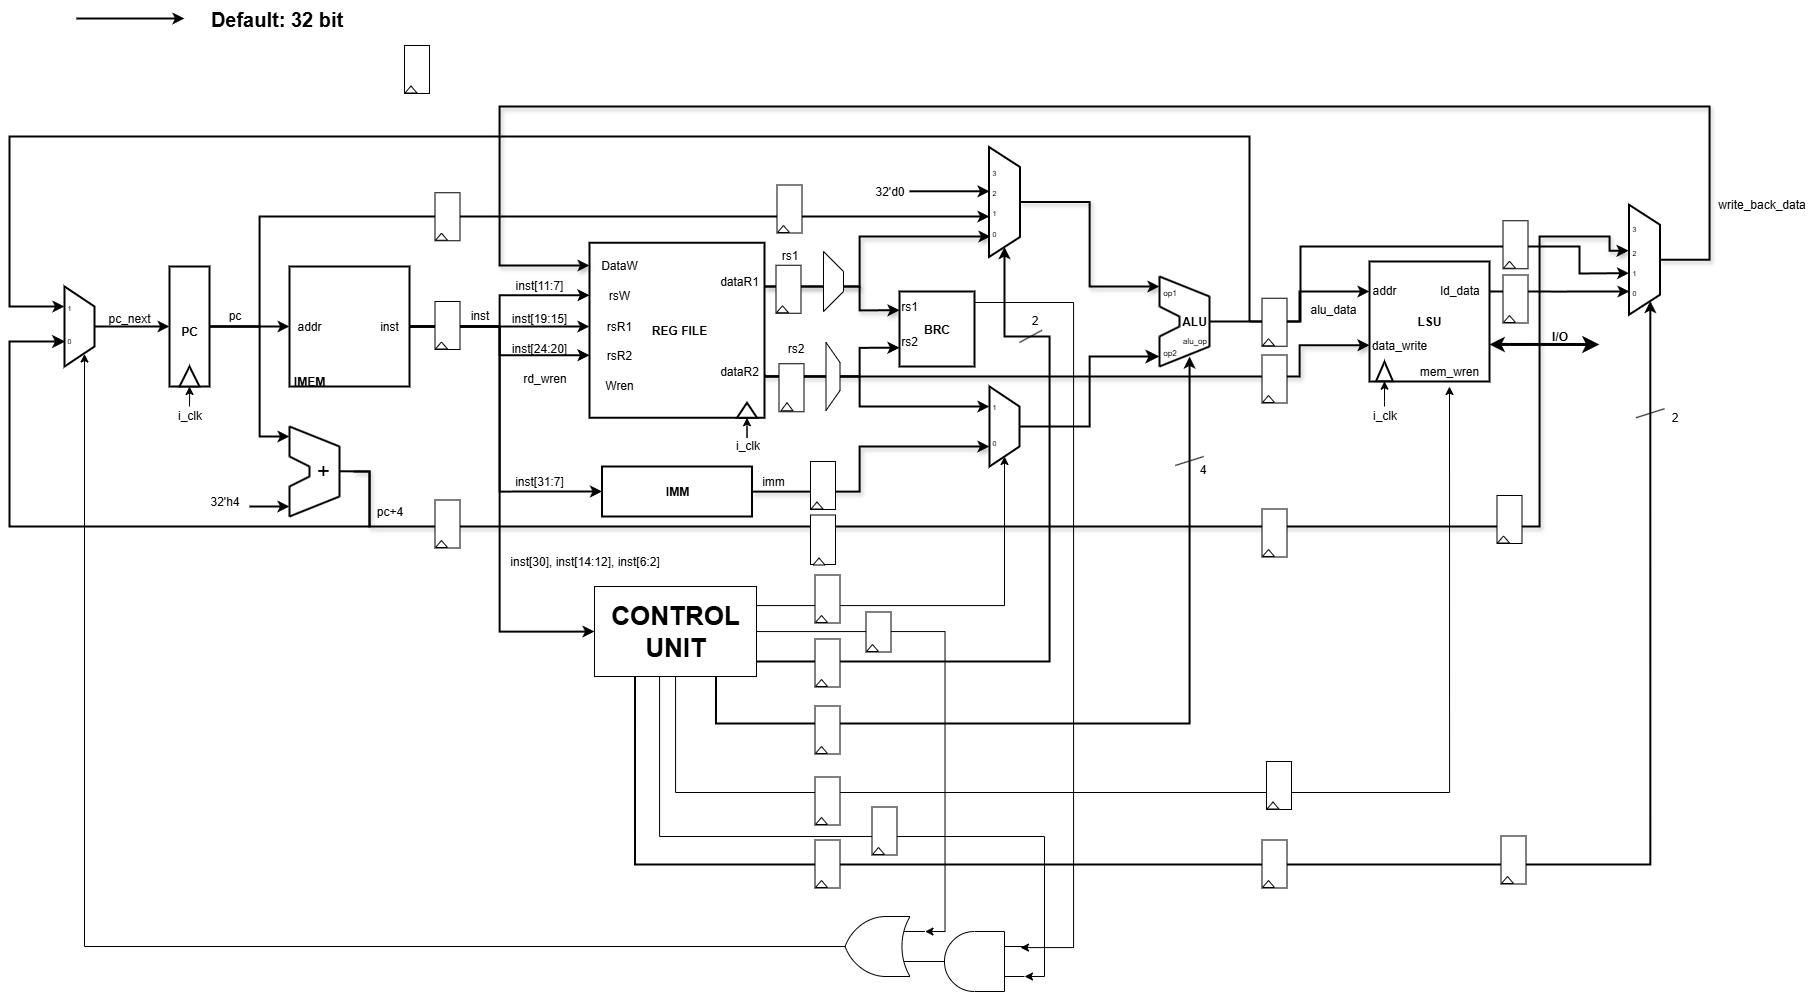
\includegraphics[width=\textwidth]{../image/Top-level_block_diagram.png}
  \caption{Five-stage scalar pipeline datapath of \texttt{pipelined\_vpu}}
  \label{fig:pipeline_datapath}
\end{figure}

\textbf{Instruction Fetch (IF).} The program counter \texttt{pc} is a 32-bit
synchronous register that resets to zero. It advances by 4 each cycle unless a stall
or branch-taken condition is asserted. Instruction memory (\texttt{imem\_sync}) is a
synchronous SRAM with a one-cycle read latency; the registered output arrives directly
at the ID stage, eliminating a redundant IF/ID instruction register. On a branch taken
or jump (\texttt{pc\_sel}), the IF stage is flushed by injecting a NOP
(\texttt{32'h0000\_0013}, \texttt{ADDI x0,x0,0}) into \texttt{imem\_sync}'s output
register.

\textbf{Instruction Decode (ID).} The control unit decodes the 11-bit pattern
\texttt{\{instr[30], instr[14:12], instr[6:0]\}} and generates the full set of control
signals: \texttt{br\_ctrl}, \texttt{j\_taken}, \texttt{ImmSel}, \texttt{alu\_op},
\texttt{wb\_sel}, \texttt{mem\_wren}, \texttt{rd\_wren}, \texttt{is\_load}, and
\texttt{is\_vector}. The register file is read combinatorially; two bypass muxes
(\texttt{rf1\_fwd}, \texttt{rf2\_fwd}) apply the WB result to the register-file output
in the same cycle to avoid a write-before-read race.

\textbf{Execute (EX).} The ALU computes the result using a 4-bit opcode
(\texttt{alu\_op\_exe}). Operand-A is selected between \texttt{rs1\_data} (forwarded)
and the EX-stage PC (\texttt{pce}) via \texttt{opa\_sel\_exe}; operand-B is selected
between forwarded \texttt{rs2\_data} and the sign-extended immediate via
\texttt{opb\_sel\_exe}. A separate branch comparator (\texttt{brc}) evaluates the
branch condition using the forwarded operands without consuming the ALU.

\textbf{Memory (MEM).} Load and store instructions access \texttt{dmem\_sync} through
the scalar port. The IO region (\texttt{addr[31:16] == 0x1000}) is handled inline:
writes update local registers (\texttt{ledr\_r}, \texttt{ledg\_r}, etc.); reads return
the corresponding register values. UART-mapped addresses (\texttt{addr[31:8] == 0xFF0000})
are decoded at the top level and steered away from \texttt{dmem\_sync}.

\textbf{Write-Back (WB).} A 2-bit selector \texttt{wb\_sel\_wb} chooses between load
data (0), ALU result (1), PC+4 (2), or immediate (3). Load-data sign and zero extension
is computed combinatorially based on \texttt{func3\_wb} and the low-order address bits
\texttt{addr\_lo\_wb}. Byte and half-word loads are supported (\texttt{LB}, \texttt{LH},
\texttt{LBU}, \texttt{LHU}).

\subsection{Hazard Detection}
\label{subsec:hazard}

Two independent hazard conditions require pipeline stalls or flushes.

\textbf{Load-use hazard.} When a load instruction (\texttt{is\_load\_exe = 1}) is in
the EX stage and the immediately following instruction in ID reads the same destination
register, the result is not available for forwarding in time. The detection condition is:

\begin{equation}
\mathit{stall\_ld} = \mathit{is\_load\_exe} \;\wedge\; (\mathit{rd\_exe} \neq \mathbf{0})
  \;\wedge\; (\mathit{rd\_exe} = \mathit{rs1_{ID}} \;\vee\; \mathit{rd\_exe} = \mathit{rs2_{ID}})
\label{eq:load_use}
\end{equation}

When \texttt{stall\_ld} is asserted, the PC register and IF/ID pipeline registers are
held (\texttt{stall = 1}) and a bubble is injected into the ID/EX registers by
zeroing all control signals in the \texttt{hazard} path.

\textbf{VPU dispatch stall.} When a vector instruction reaches the EX stage
(\texttt{is\_vector\_exe = 1}) and the \gls{vpu} signals it is not ready
(\texttt{vpu\_ready\_i = 0}), the entire pipeline is held:

\begin{equation}
\mathit{vpu\_stall} = \mathit{is\_vector\_exe} \;\wedge\; \neg\,\mathit{vpu\_ready\_i}
\label{eq:vpu_stall}
\end{equation}

All pipeline registers from PC through MEM/WB are clock-enabled with
\texttt{!vpu\_stall}, so the entire pipeline freezes until \texttt{vpu\_ready\_i} goes
high. This simple freeze-and-hold approach is correct because the vector instruction
itself is already in the EX stage driving \texttt{vpu\_insn\_o} and \texttt{vpu\_rs1/rs2\_data\_o};
the \gls{vpu} latches these on the first cycle that \texttt{vpu\_ready} is high.

\subsection{Data Forwarding}
\label{subsec:forwarding}

Full EX$\to$MEM and MEM$\to$WB forwarding bypasses are implemented to avoid
unnecessary stalls for back-to-back ALU instructions. The forwarding priority for
operand A of the EX stage is:

\begin{enumerate}
  \item \texttt{fwd\_a = 2'b01}: Forward from EX/MEM register (\texttt{alu\_result\_m})
        when the MEM-stage instruction writes the same register as rs1 in EX.
  \item \texttt{fwd\_a = 2'b10}: Forward from the WB writeback path (\texttt{rf\_wdata})
        when the WB-stage instruction writes rs1 in EX.
  \item \texttt{fwd\_a = 2'b00}: Use the ID/EX register value directly.
\end{enumerate}

The same priority chain applies to operand B (\texttt{fwd\_b}). Forwarding from
\texttt{rf\_wdata} rather than the MEM/WB register output is intentional: it picks up
VPU configuration writebacks (Section~\ref{subsec:vpu_dispatch}) transparently.

\subsection{VPU Dispatch Protocol}
\label{subsec:vpu_dispatch}

When the control unit decodes an OP-V opcode (\texttt{is\_vector = 1}), the instruction
propagates to the EX stage in the normal fashion. In the EX stage, the core continuously
drives \texttt{vpu\_insn\_vld\_o = is\_vector\_exe} and presents the instruction word
plus forwarded operands on \texttt{vpu\_insn\_o}, \texttt{vpu\_rs1\_data\_o}, and
\texttt{vpu\_rs2\_data\_o}.

The \gls{vpu} accepts the instruction when it asserts \texttt{vpu\_ready}; simultaneously,
the scalar pipeline resumes. If the \gls{vpu} deasserts \texttt{vpu\_ready} (FIFO full
or \gls{vlsu} busy), the pipeline stalls via \texttt{vpu\_stall} until acceptance.

A special case applies to \texttt{vsetvl}/\texttt{vsetvli} instructions
(\texttt{is\_cfg\_exe}). These must write the new \texttt{vl} value back to a scalar
general-purpose register (\texttt{rd}). Because the \gls{vpu} updates its internal CSR
asynchronously over several cycles, the scalar core captures the destination register
address (\texttt{rd\_addr\_exe}) in a pending register (\texttt{vpu\_cfg\_rd\_r}) and
waits for the \texttt{vpu\_cfg\_done\_i} pulse. When \texttt{vpu\_cfg\_done\_i} arrives,
the RF write port is overridden:

\begin{lstlisting}[language=SV, caption={VPU config writeback in WB stage},
                   label={lst:cfg_wb}]
always_comb begin
    if (vpu_cfg_done_i && vpu_cfg_pending_r && vpu_cfg_rd_r != 5'b0) begin
        rf_wren  = 1'b1;
        rf_waddr = vpu_cfg_rd_r;
        rf_wdata = vpu_vl_remain_i; // actual vl from VPU CSR
    end else begin
        rf_wren  = rd_wren_wb;
        rf_waddr = rd_addr_wb;
        rf_wdata = wb_data;
    end
end
\end{lstlisting}

%% =============================================================================
\section{VPU Architecture}
\label{sec:vpu_arch}
%% =============================================================================

The \gls{vpu} subsystem is contained within \texttt{vproc\_system\_wrapper}, which
instantiates the decoder, FIFO, FSM, cycle counter, four \gls{vrf} banks, four
processor lanes, the reduction unit, the vector \gls{vlsu}, and auxiliary units
(address generator, CSR, mask enable, mask write buffer, merge unit, scalar expand).
The entire subsystem is parameterised by \texttt{NUM\_REGS}~=~32, \texttt{ADDR\_WIDTH}~=~5,
and \texttt{CTRL\_WIDTH}~=~49 (the 48-bit logical bus plus a \texttt{vsetivli} flag).

\begin{figure}[H]
  \centering
  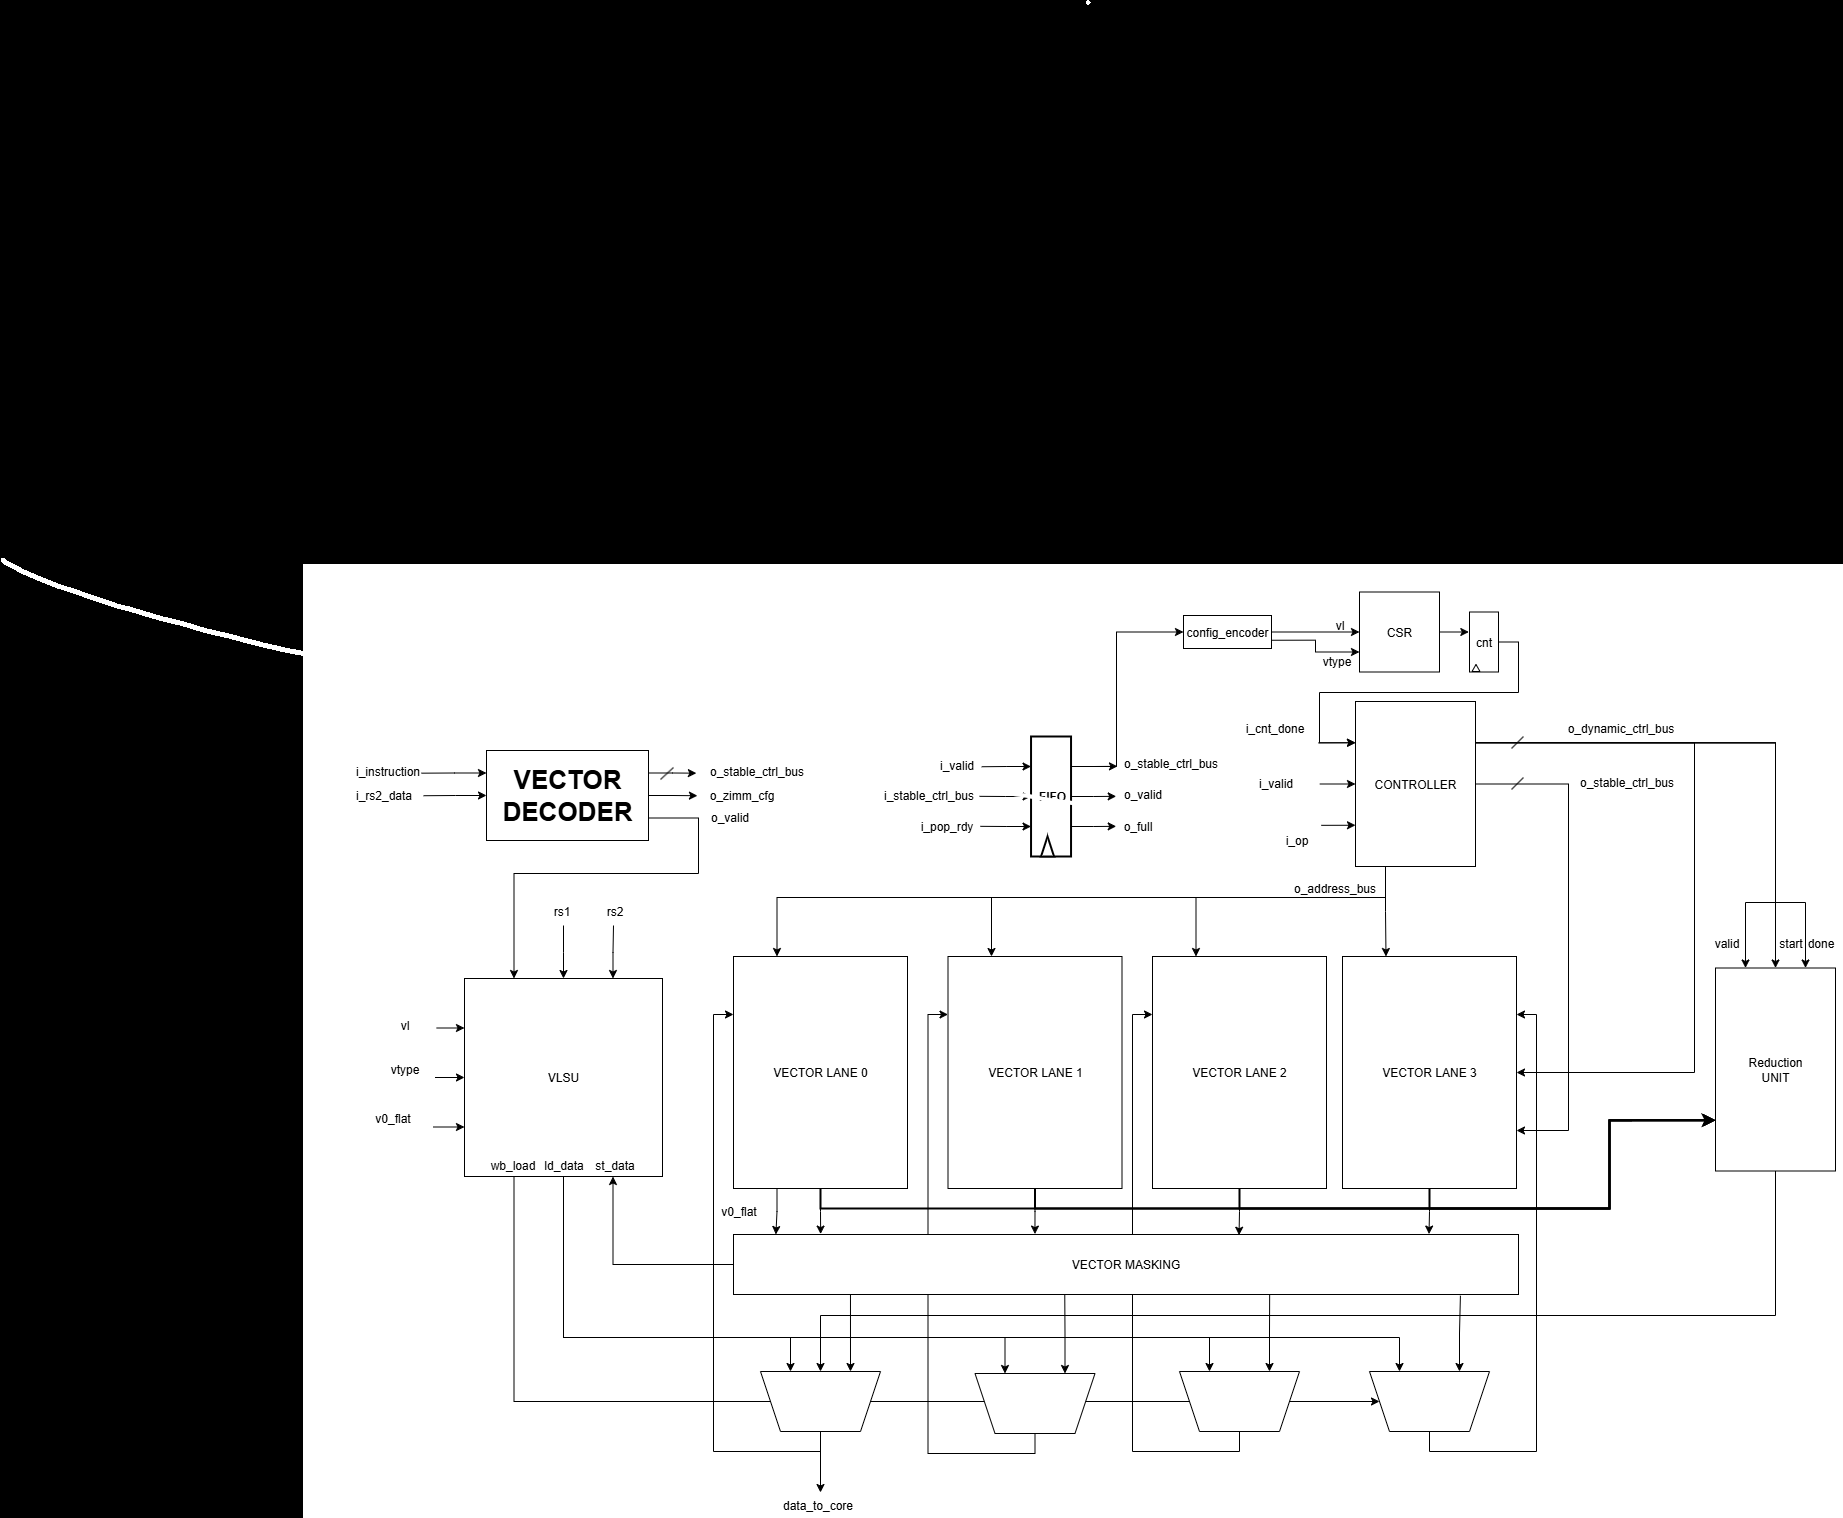
\includegraphics[width=\textwidth]{../image/vpu_top_wrapper.png}
  \caption{Block diagram of the \texttt{vproc\_system\_wrapper} VPU subsystem}
  \label{fig:vpu_wrapper}
\end{figure}

\subsection{Instruction Decoder}
\label{subsec:decoder}

The decoder module \texttt{vproc\_vdecoder} accepts a 32-bit RVV instruction word and
produces a 49-bit \texttt{ctrl\_bus} that encodes all execution control fields. The
decoding is purely combinational; the decoder also outputs a 32-bit sign-extended
immediate for \texttt{vimm*} instructions.

\subsubsection{ctrl\_bus Layout}

\begin{table}[H]
\centering
\caption{49-bit \texttt{ctrl\_bus} field encoding}
\label{tab:ctrlbus}
\begin{tabular}{clp{7cm}}
\toprule
\textbf{Bits} & \textbf{Field} & \textbf{Meaning} \\
\midrule
{[4:0]}   & \texttt{vs1\_addr}          & Source register 1 address (5-bit) \\
{[9:5]}   & \texttt{vs2\_addr}          & Source register 2 address \\
{[14:10]} & \texttt{vd\_addr}           & Destination register address \\
{[20:15]} & \texttt{funct6}             & Instruction funct6 field \\
{[21]}    & \texttt{is\_widen}          & Widening operation (result is 2$\times$ SEW) \\
{[22]}    & \texttt{is\_unsigned\_vs1}  & vs1 treated as unsigned \\
{[23]}    & \texttt{is\_unsigned\_vs2}  & vs2 treated as unsigned \\
{[24]}    & \texttt{is\_subtraction}    & Negate adder (vsub/vrsub) \\
{[25]}    & \texttt{is\_immediate}      & Use zimm/imm operand instead of vs1 \\
{[26]}    & \texttt{is\_rs1}            & Use scalar rs1 as vs1 \\
{[27]}    & \texttt{is\_mulh}           & Select upper-half multiplier product \\
{[28]}    & \texttt{is\_config}         & vsetvl/vsetvli instruction \\
{[29]}    & \texttt{is\_vector}         & OP-V opcode family \\
{[30]}    & \texttt{cfg\_is\_vsetvli}   & 1 = vsetvli, 0 = vsetvl \\
{[31]}    & \texttt{vm}                 & Mask bit from instruction [25]: 1 = unmasked \\
{[39:32]} & \texttt{vtype\_enc}         & \texttt{\{vma,vta,vsew[2:0],vlmul[2:0]\}} \\
{[40]}    & \texttt{is\_carry}          & vadc/vsbc with carry from v0 \\
{[41]}    & \texttt{is\_mask\_carry}    & vmadc/vmsbc — result is a carry mask \\
{[42]}    & \texttt{is\_masking}        & Mask-generating instruction (vmseq, etc.) \\
{[43]}    & \texttt{is\_final\_masking} & Requires ST\_FINAL\_MASKING commit phase \\
{[44]}    & \texttt{is\_reverse\_sub}   & vrsub: swap minuend/subtrahend \\
{[45]}    & \texttt{minmax\_is\_min}    & 1 = vmin/vminu; 0 = vmax/vmaxu \\
{[46]}    & \texttt{minmax\_is\_unsign} & 1 = unsigned comparison for min/max \\
{[47]}    & \texttt{is\_reduction}      & vred* instruction \\
{[48]}    & \texttt{cfg\_is\_vsetivli}  & 1 = vsetivli (AVL from 5-bit immediate) \\
\bottomrule
\end{tabular}
\end{table}

\subsubsection{Decoding Categories}

The decoder classifies every instruction into one of five execution categories, which
determine the \gls{fsm} state sequence:

\begin{description}
  \item[Config (\texttt{is\_config}).] Instructions \texttt{vsetvl}, \texttt{vsetvli},
    and \texttt{vsetivli} update the CSR registers \texttt{vl} and \texttt{vtype}.
    No \gls{vrf} access occurs; the \gls{fsm} traverses ST\_IDLE $\to$ ST\_CONFIG $\to$
    ST\_IDLE in a single cycle.
  \item[Masking (\texttt{is\_masking}).] Instructions such as \texttt{vmseq.vv},
    \texttt{vmslt.vv}, and \texttt{vmadc.vv} produce a 1-bit result per element that
    is packed into a destination mask register. The \gls{fsm} accumulates comparison
    bits over multiple cycles (ST\_MASKING) then writes the complete packed result in
    one cycle (ST\_FINAL\_MASKING).
  \item[Widening (\texttt{is\_widen}).] Two-cycle widening instructions (e.g.,
    \texttt{vaddw.vv}) alternate between ST\_WIDENL (write low half) and ST\_WIDENH
    (write high half) until all elements are processed.
  \item[Reduction (\texttt{is\_reduction}).] Instructions \texttt{vredsum.vs},
    \texttt{vredmax.vs}, etc. use the dedicated reduction unit in a serial
    accumulation loop (ST\_REDUCTION $\to$ ST\_REDUCTION\_DONE).
  \item[Exec (default).] All remaining arithmetic, logical, shift, multiply, and
    min/max instructions execute in ST\_EXEC, advancing one 32-bit chunk per cycle.
\end{description}

\subsubsection{Compare Group Decode}

The compare group (\texttt{funct6[5:3] == 3'b011}) requires the \texttt{is\_masking}
and \texttt{is\_final\_masking} flags to be set. The relevant decoder logic is:

\begin{lstlisting}[language=SV,
  caption={Compare group detection in \texttt{vproc\_vdecoder} (representative extract)},
  label={lst:cmp_decode}]
// Compare group: funct6[5:3] == 3'b011
wire is_cmp = (funct6[5:3] == 3'b011);

// Masking: compare instructions and vmadc/vmsbc
assign ctrl_bus[42] = is_cmp || (funct6 == 6'b010001) || (funct6 == 6'b010011);
// Final masking: always paired with masking for compare
assign ctrl_bus[43] = ctrl_bus[42];
\end{lstlisting}

\subsection{Instruction FIFO}
\label{subsec:fifo}

The \texttt{vproc\_fifo} module is a synchronous circular buffer with the following
parameters: DEPTH~=~8 entries, CTRL\_WIDTH~=~49, RS1\_WIDTH~=~32, IMM\_WIDTH~=~32.
Each entry therefore holds $49 + 32 + 32 = 113$ bits. At eight entries, the FIFO
can absorb a burst of eight consecutive vector instructions while the \gls{vpu} is
executing the first, preventing unnecessary scalar stalls.

\textbf{Push protocol.} The scalar core pushes on each cycle that a valid OP-V
instruction is presented (\texttt{push\_valid \&\& !is\_full}). Config instructions
(\texttt{is\_config = 1}) bypass the \texttt{vpu\_ready} guard and push whenever the
FIFO has space; this is necessary because a \texttt{vsetvl*} issued while the VLSU
is busy must still reach the \gls{vpu} without waiting for the VLSU to finish.
All other instructions push only when \texttt{vpu\_ready} is high, preventing
duplicate entries when the scalar pipeline re-presents the same instruction after
a stall.

\textbf{Pop protocol.} The \gls{fsm} asserts \texttt{pop\_ready} during ST\_IDLE when
it latches a new instruction. The FIFO advances its read pointer, and the next entry
becomes visible one cycle later.

\textbf{Combinational loop elimination.} An earlier design connected the FIFO's output
directly to its input (forwarding bypass), creating a 143-node combinational path:
\texttt{push\_valid $\to$ forwarding $\to$ fifo\_full $\to$ vpu\_ready $\to$ push\_valid}.
This path limited the achievable $F_{\max}$ to 16.7~MHz. The bypass was removed; all
FIFO outputs are purely registered. The cost is one additional dispatch-latency cycle
when the FIFO is empty, which is negligible because every vector instruction requires
multiple execution cycles anyway.

\subsection{Execution FSM}
\label{subsec:fsm}

The \gls{fsm} in \texttt{vproc\_fsm} is the central sequencer of the \gls{vpu}
execution pipeline. It consists of nine states encoded as a 4-bit binary enumeration.

\subsubsection{State Diagram}

\begin{figure}[H]
\centering
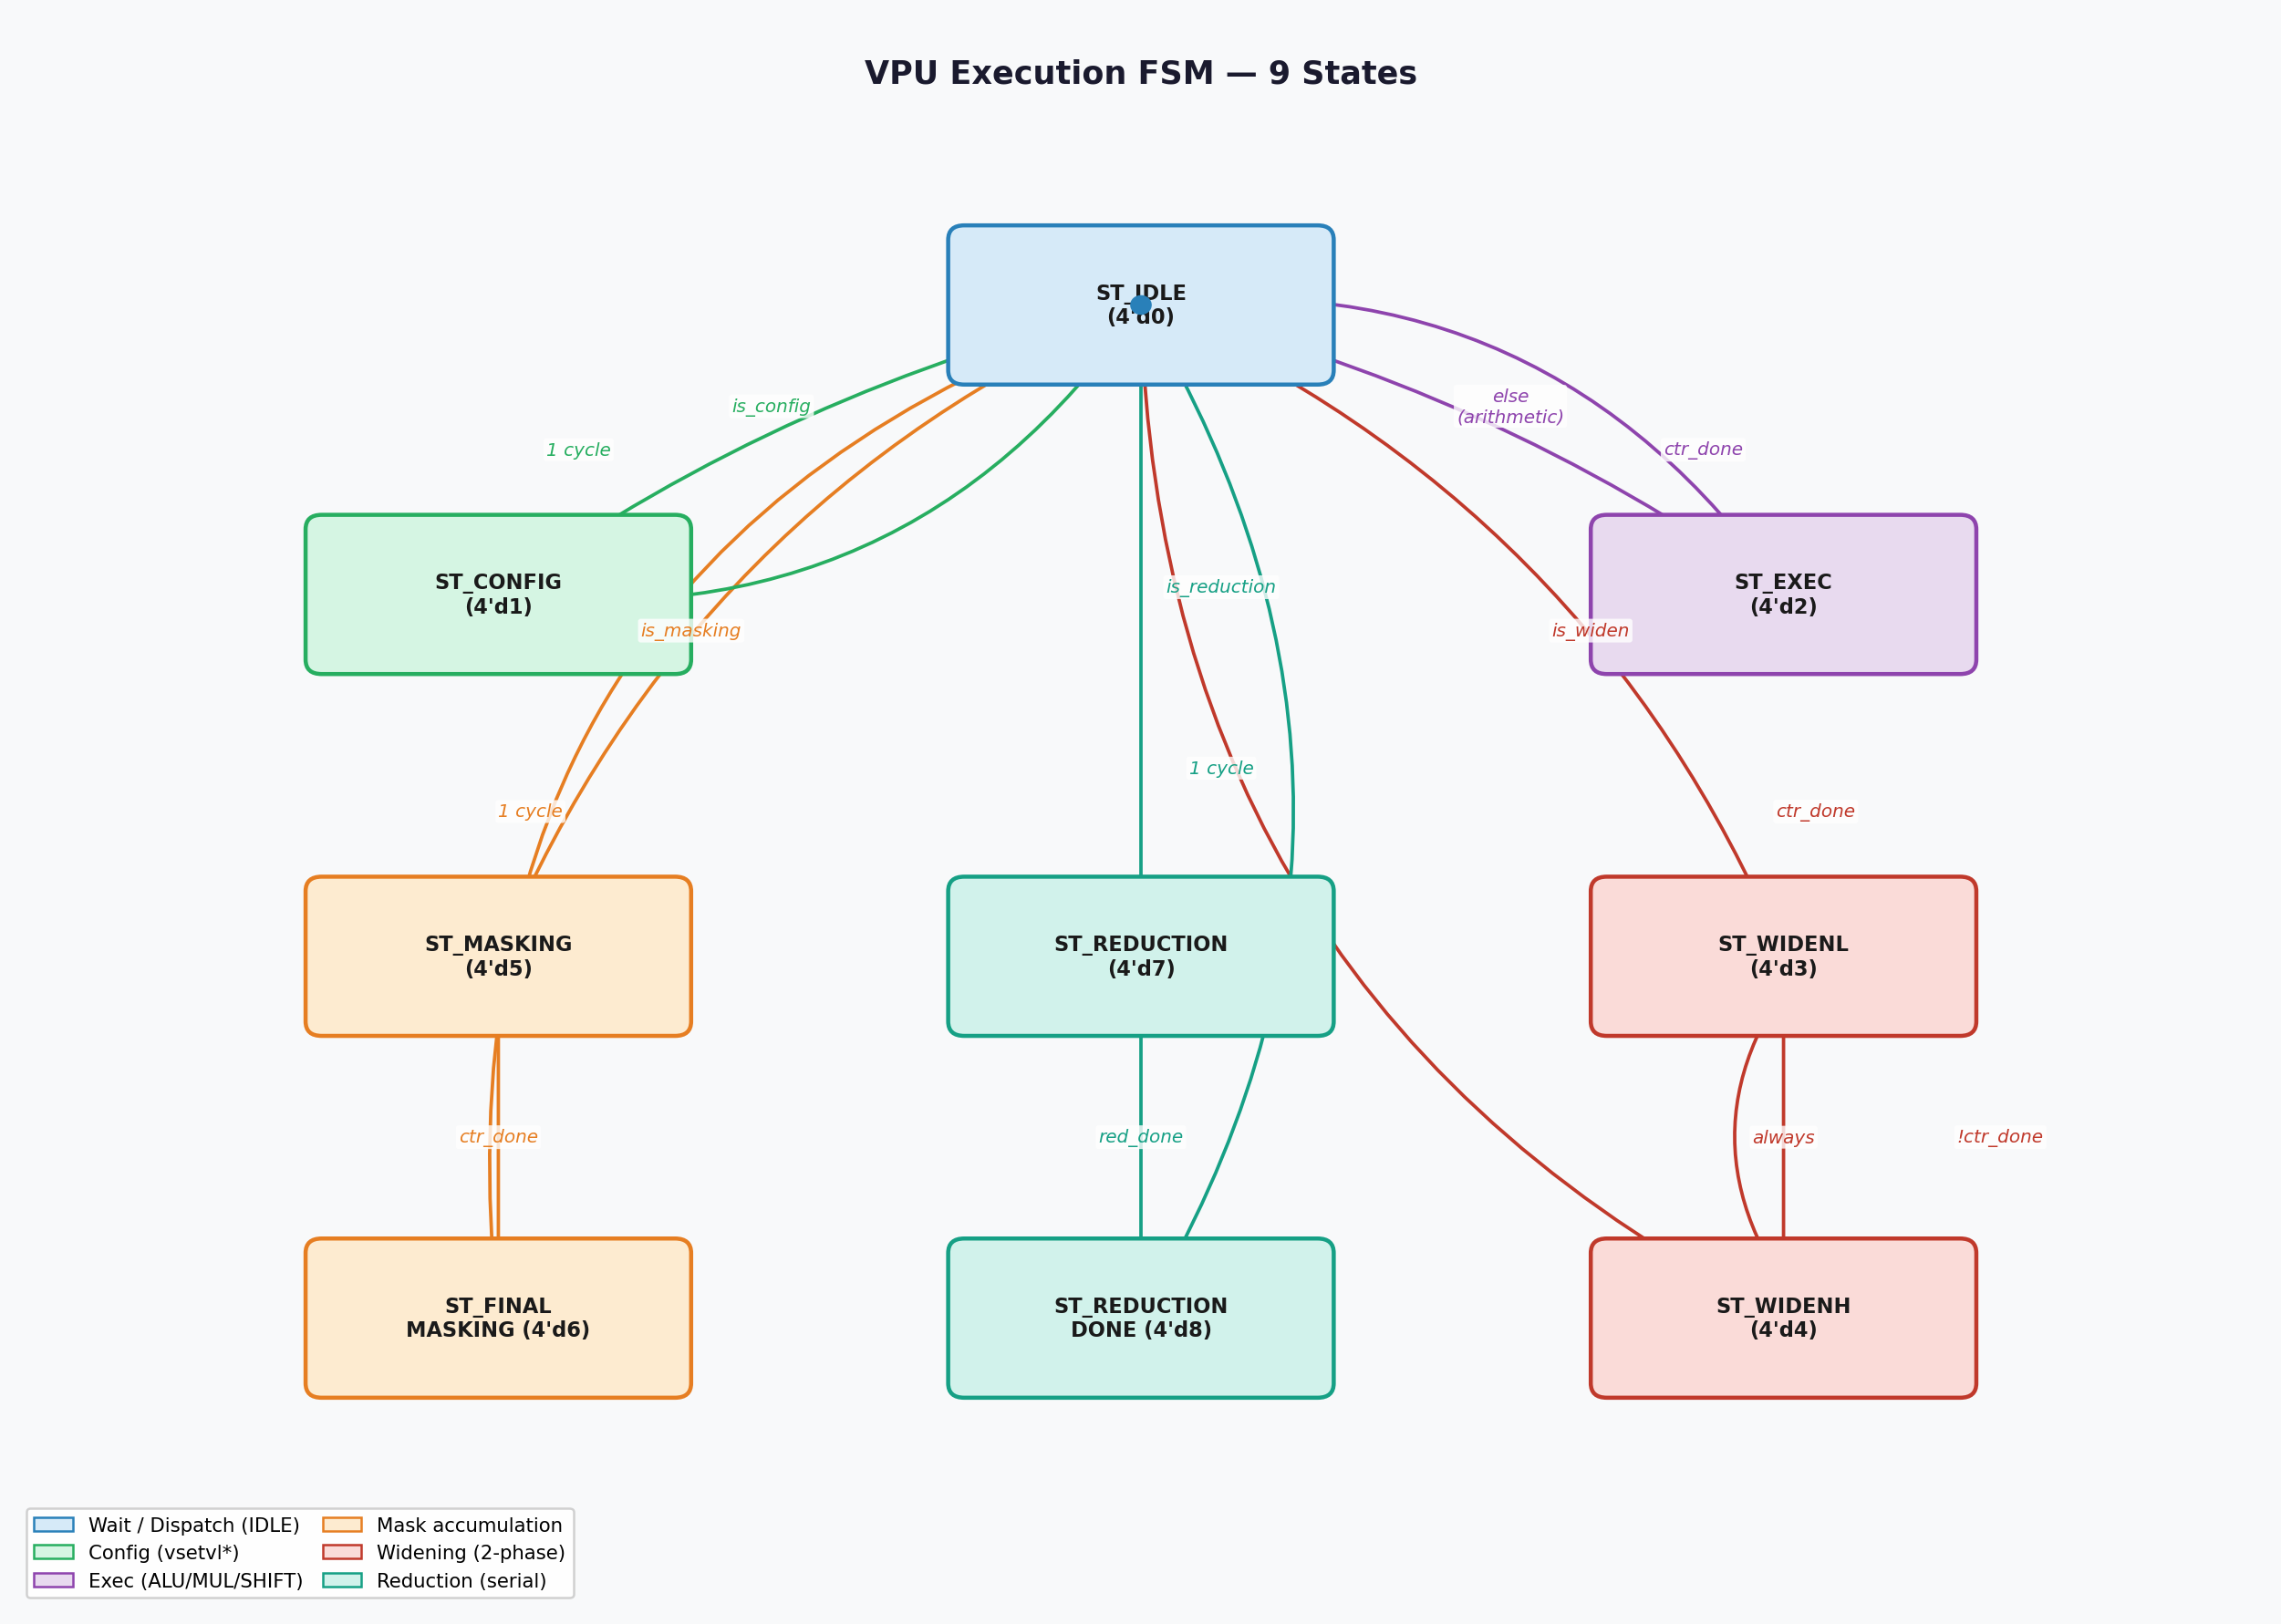
\includegraphics[width=\textwidth]{../image/fsm_diagram.png}
\caption{VPU execution \gls{fsm} state diagram (nine states). ST\_IDLE is the central
         dispatch hub; each instruction category routes to a dedicated execution state.
         All paths return to ST\_IDLE within one extra cycle after completion.}
\label{fig:fsm_states}
\end{figure}

\subsubsection{Output Encoding}

\begin{table}[H]
\centering
\caption{FSM output signals asserted in each state}
\label{tab:fsm_outputs}
\begin{tabular}{lccccccccc}
\toprule
\textbf{Signal} &
\rotatebox{70}{\textbf{ST\_IDLE}} &
\rotatebox{70}{\textbf{ST\_CONFIG}} &
\rotatebox{70}{\textbf{ST\_EXEC}} &
\rotatebox{70}{\textbf{ST\_WIDENL}} &
\rotatebox{70}{\textbf{ST\_WIDENH}} &
\rotatebox{70}{\textbf{ST\_MASKING}} &
\rotatebox{70}{\textbf{ST\_FINAL\_MASKING}} &
\rotatebox{70}{\textbf{ST\_REDUCTION}} &
\rotatebox{70}{\textbf{ST\_REDUCTION\_DONE}} \\
\midrule
\texttt{offset\_reset}   & \checkmark &   &   &   &   &   &   &   &   \\
\texttt{latch\_ctrl\_en} & (*)  &   &   &   &   &   &   &   &   \\
\texttt{pop\_ready}      & (*)  &   &   &   &   &   &   &   &   \\
\texttt{counter\_start}  & (*) &   &   &   &   &   &   &   &   \\
\texttt{reduction\_start}& (*r) &   &   &   &   &   &   &   &   \\
\texttt{csr\_cfg\_en}    &   & \checkmark &   &   &   &   &   &   &   \\
\texttt{vrf\_wren}       &   &   & \checkmark & \checkmark & \checkmark &   & \checkmark &   & \checkmark \\
\texttt{s\_offset\_en}   &   &   & \checkmark &   & \checkmark & \checkmark &   & (**) &   \\
\texttt{d\_offset\_en}   &   &   & \checkmark & \checkmark & \checkmark &   &   &   &   \\
\texttt{widen\_sel}      &   &   &   &   & \checkmark &   &   &   &   \\
\texttt{reduction\_en}   &   &   &   &   &   &   &   & (**) &   \\
\bottomrule
\multicolumn{10}{l}{\footnotesize (*) Conditional on \texttt{instr\_valid}. (*r) Conditional on \texttt{instr\_valid \&\& is\_reduction}.} \\
\multicolumn{10}{l}{\footnotesize (**) Conditional on \texttt{!reduction\_busy}.} \\
\end{tabular}
\end{table}

\subsubsection{Cycle Count per Instruction Type}

The number of execution cycles for a vector instruction depends on the active
element count and SEW. Let $N_{elem}$ be the total number of active elements
(the value of \texttt{vl}). The number of 32-bit chunks processed per clock cycle
is $C_{per} = 32 / \mathit{SEW}$ (4 for SEW=8, 2 for SEW=16, 1 for SEW=32).
The execution cycle count for non-reduction instructions is therefore:

\begin{equation}
  T_{exec} = \left\lceil \frac{N_{elem}}{C_{per}} \right\rceil
  \label{eq:exec_cycles}
\end{equation}

For reduction instructions, the serial accumulation within \texttt{vproc\_reduction}
adds $C_{per}$ cycles per chunk (one clock per element), so the total is:

\begin{equation}
  T_{red} = \left\lceil \frac{N_{elem}}{C_{per}} \right\rceil \times C_{per} + 1
           = N_{elem} + 1
  \label{eq:red_cycles}
\end{equation}

with the $+1$ accounting for the ST\_REDUCTION\_DONE write cycle.

\subsection{Vector Register File}
\label{subsec:vrf}

The vector register file consists of 32 registers, each 128 bits wide, implemented as
four parallel 8-bit bank instances of \texttt{vproc\_vregfile}. Each bank instance
stores 32 words of 8 bits, provides two asynchronous read ports (\texttt{vs1},
\texttt{vs2}), and one synchronous write port (\texttt{vd}) with a per-byte write
enable (\texttt{write\_en}). The four banks together deliver a 32-bit \texttt{rs1\_data}
and \texttt{rs2\_data} per cycle to one execution lane.

Each of the four \gls{vrf} instances in \texttt{vproc\_system\_wrapper} serves one
execution lane. Because the processor lane operates on one 32-bit chunk per cycle, the
four instances in parallel provide the full 128-bit register content to the four lanes
simultaneously. This replication is preferred over a single wide \gls{vrf} with
serialisation logic because it minimises the critical-path depth on the read side and
permits independent byte-enable gating on each lane.

\textbf{LMUL grouping.} For LMUL~$>$~1, consecutive register numbers form a logical
group. For example, LMUL~=~4 with base register \texttt{v8} occupies physical registers
\texttt{v8}, \texttt{v9}, \texttt{v10}, \texttt{v11}. The \gls{vrf} address generator
(Section~\ref{subsec:addr_gen}) increments the effective address by one each cycle,
automatically traversing the entire group without explicit instruction control.

\textbf{Read-write timing.} Register reads are asynchronous (combinational). Register
writes are synchronous, occurring on the rising clock edge when the corresponding
\texttt{write\_en} bit is asserted. There is no write-then-read forwarding within the
\gls{vrf}; the \gls{fsm} and hazard scoreboard in the wrapper guarantee that an
in-flight load completes before the same register is read by an OP-V instruction.

The dedicated \texttt{mask\_data} port provides a fixed asynchronous read of register
\texttt{v0} for all four banks; this 128-bit flat mask is used by the mask-enable unit
and the \gls{vlsu}.

\subsection{VRF Address Generator}
\label{subsec:addr_gen}

The \texttt{vproc\_vrf\_addr\_gen} module maintains two independent offset counters:
\texttt{s\_offset\_r} for source addresses (vs1, vs2) and \texttt{d\_offset\_r} for
the destination address (vd). Both counters are reset to zero by \texttt{offset\_clear}
(asserted in ST\_IDLE) and incremented by one each cycle when the corresponding enable
signal is asserted.

The effective addresses are computed combinatorially:

\begin{equation}
\begin{aligned}
\mathit{vs1\_addr} &= \mathit{vs1\_base} + \mathit{s\_offset\_r} \\
\mathit{vs2\_addr} &= \mathit{vs2\_base} + \mathit{s\_offset\_r} \\
\mathit{vd\_addr}  &= \mathit{vd\_base}  + \mathit{d\_offset\_r}
\end{aligned}
\label{eq:vrf_addr}
\end{equation}

The independence of \texttt{s\_offset\_r} and \texttt{d\_offset\_r} is essential for
widening instructions: during ST\_WIDENL, only \texttt{d\_offset\_en} is asserted
(destination advances); during ST\_WIDENH, both offsets advance. This produces the
correct interleaving where one source chunk generates two destination writes (low
half and high half in consecutive destination registers).

The 5-bit counter width matches \texttt{ADDR\_WIDTH = 5} (up to 32 distinct addresses),
so the address wraps naturally for LMUL~=~8 without overflow guard logic.

\subsection{Execution Lane}
\label{subsec:exec_lane}

The module \texttt{vproc\_processor\_lane} is instantiated four times in
\texttt{vproc\_system\_wrapper}, one per 32-bit lane. All four instances receive
identical control signals and independent 32-bit data words from the four \gls{vrf}
banks, operate in parallel, and write their results back to their respective bank.

\subsubsection{Lane Datapath}

\begin{figure}[H]
  \centering
  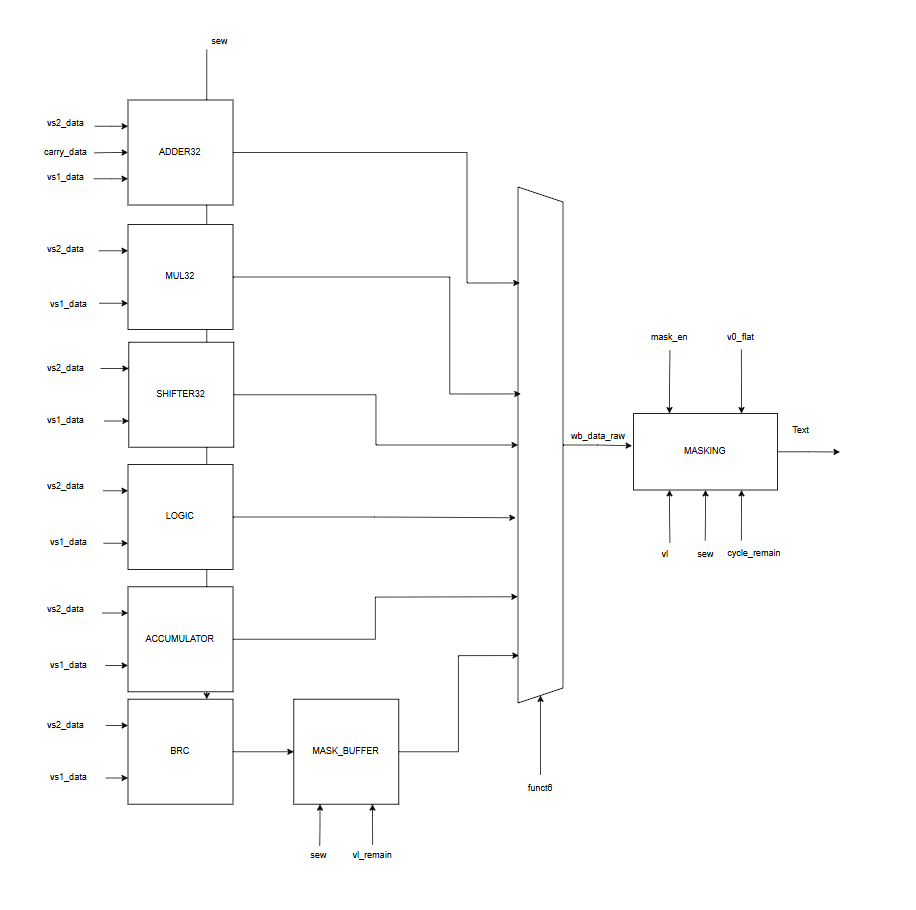
\includegraphics[width=\textwidth]{../image/executing_lane.png}
  \caption{Execution lane block diagram of \texttt{vproc\_processor\_lane}: operand
           muxes, seven parallel functional units, result selection mux, and mask
           application stage.}
  \label{fig:exec_lane}
\end{figure}

\textbf{SEW slicing.} Although the \gls{vrf} is VLEN~=~128 bits wide, each lane
processes exactly one 32-bit chunk per cycle. The SEW (element width) determines
how many independent operations are packed into that 32-bit chunk: four 8-bit
operations for SEW=8 (e8), two 16-bit for SEW=16 (e16), or one 32-bit for SEW=32
(e32). All functional units receive the full 32-bit chunk and decompose it internally
according to the \texttt{sew} input.

\textbf{Mask application.} When the instruction has \texttt{vm = 0} (masked),
the per-lane write enable \texttt{lane\_we[3:0]} is derived from the corresponding
bits of v0 by the mask-enable unit. Within the lane, an additional software-visible
mask is applied by AND-ing the result with \texttt{lane\_mask\_32}, which expands
each mask bit to cover the full width of its element:

\begin{equation}
\mathit{wb\_result} = \mathit{wb\_unmasked} \;\mathbin{\&}\; \mathit{lane\_mask\_32}
\label{eq:lane_mask}
\end{equation}

where \texttt{lane\_mask\_32} is $\{8 \times \mathit{vmask[3]}, 8 \times \mathit{vmask[2]},
8 \times \mathit{vmask[1]}, 8 \times \mathit{vmask[0]}\}$ for SEW=8, and correspondingly
expanded for SEW=16 and SEW=32.

\subsection{Arithmetic and Logic Units}
\label{subsec:alu_units}

\subsubsection{Adder (\texttt{vproc\_adder})}

The adder supports three lane configurations depending on \texttt{sew}: four
independent 8-bit operations, two independent 16-bit operations, or one 32-bit
operation. Each sub-operation is computed with a carry-save structure that prevents
carry propagation between lanes:

\begin{lstlisting}[language=SV,
  caption={Independent 8-bit lane computation in \texttt{vproc\_adder}},
  label={lst:adder_8b}]
tmp8_0 = {1'b0, op_a[7:0]} +
         {1'b0, (sub ? ~op_b[7:0] : op_b[7:0])} +
         adder_third_1b(sub, use_carry, carry_in[0]);
\end{lstlisting}

The \texttt{adder\_third\_1b} function encodes the carry-in / borrow-in logic:
for addition with \texttt{use\_carry}, it passes \texttt{carry\_in[i]} directly;
for subtraction with \texttt{use\_carry}, it passes the complement (\texttt{$\sim$carry\_in[i]});
for plain subtraction (vsub), it passes \texttt{1'b1} (two's complement). This covers
all four instruction variants: \texttt{vadd}, \texttt{vsub}, \texttt{vadc}, and
\texttt{vsbc}.

The adder also produces a widening result: \texttt{result\_lo} holds the truncated
output and \texttt{result\_hi} holds the sign- or zero-extension of the most significant
bit, selected by the \texttt{unsign} flag.

\subsubsection{Multiplier (\texttt{vproc\_mul})}

The multiplier supports three instruction variants:
\begin{itemize}
  \item \textbf{VMUL}: lower 32-bit product, all lane widths.
  \item \textbf{VMULH, VMULHU, VMULHSU}: upper half of the $2\times\mathit{SEW}$ product,
        used by the processor lane when \texttt{is\_mulh = 1} or \texttt{widen\_sel = 1}.
  \item \textbf{Widening multiply (VMULW/VMULWU/VMULWSU)}: the full $2\times\mathit{SEW}$
        product split between \texttt{mul\_lo} (lower half) and \texttt{mul\_hi} (upper half).
\end{itemize}

The processor lane selects the appropriate output:

\begin{equation}
\mathit{result\_mul} = \begin{cases}
  \mathit{mul\_hi} & \text{if } \mathit{is\_mulh} \vee \mathit{widen\_sel} \\
  \mathit{mul\_lo} & \text{otherwise}
\end{cases}
\end{equation}

\subsubsection{Shifter (\texttt{vproc\_shifter})}

Shifts support vsll (logical left), vsrl (logical right), and vsra (arithmetic right)
for all three SEW values. The shift amount is masked to prevent out-of-range shifts:
for SEW=8 the shift amount is masked to bits [2:0] (0--7); for SEW=16 to bits [3:0]
(0--15); for SEW=32 to bits [4:0] (0--31). This masking is performed within the
shifter to match the RVV specification requirement that only the low $\log_2(\mathit{SEW})$
bits of the shift amount are used.

\subsubsection{Logic Unit (\texttt{vproc\_logic})}

The logic unit is structurally the simplest functional unit: it computes bitwise AND,
OR, and XOR on the full 32-bit lane operands simultaneously. The processor lane selects
the appropriate output via the \texttt{funct6} mux. Because the operations are bitwise,
there is no SEW dependence; a 32-bit VAND on an e8 lane is equivalent to four
independent 8-bit ANDs.

\subsubsection{Comparator (\texttt{vproc\_compare})}

The comparator produces a 4-bit \texttt{cmp\_result} vector, where each bit corresponds
to one element in the lane. The comparison type (equal, less-than, less-than-unsigned)
is encoded by \texttt{is\_less\_than} and \texttt{is\_unsign}. Note that vmseq and
vmsne are handled by equality comparison with optional inversion; vmsle, vmsleu, vmsge,
vmsgeu are synthesised from the other two primitives at the decoder level.

The 4-bit output is routed through \texttt{mask\_result\_out} to the mask write buffer
in the wrapper, which accumulates comparison bits over multiple cycles into a 128-bit
mask register. The final packed mask is written to the destination register in a single
ST\_FINAL\_MASKING cycle.

\subsubsection{Min/Max Unit (\texttt{vproc\_minmax})}

The min/max unit evaluates one comparison per element lane and selects the winner via a
2:1 mux. Four independent comparisons run in parallel for SEW=8, two for SEW=16, and
one for SEW=32. Both signed and unsigned comparisons are supported (\texttt{is\_unsign}).

\subsection{Reduction Unit}
\label{subsec:reduction}

\subsubsection{Design Rationale}

An initial prototype of the reduction unit instantiated a tree of 15 adders in parallel
to process all 16 elements of an e8 vector simultaneously. Post-synthesis timing
analysis revealed a critical path of approximately 64~ns (spanning five adder stages),
limiting the maximum clock frequency to 15.6~MHz — well below the target of 50~MHz.
The design was replaced with a serial, one-element-per-cycle accumulator that adds a
single adder to the critical path (approximately 4~ns for a 32-bit addition).
The latency cost is $N_{elem} - 1$ additional cycles per reduction instruction, which
is acceptable because the primary optimisation target is timing closure rather than
throughput for this particular instruction class.

\subsubsection{Interface Protocol}

The reduction unit exposes the following handshake protocol to the surrounding \gls{fsm}:

\begin{itemize}
  \item \textbf{start}: Asserted for one cycle by the \gls{fsm} in ST\_IDLE when a
    reduction instruction is dispatched. Resets the accumulator to zero.
  \item \textbf{valid}: Asserted by the \gls{fsm} in ST\_REDUCTION on each cycle that
    the next 128-bit chunk is ready (conditioned on \texttt{!reduction\_busy}).
  \item \textbf{busy}: Asserted internally by the reduction unit while it is iterating
    over the elements in the current chunk. The \gls{fsm} holds \texttt{s\_offset\_en}
    and \texttt{reduction\_en} low while \texttt{busy} is high.
  \item \textbf{done}: Asserted by the \gls{fsm} on the final \texttt{valid} pulse
    (when \texttt{counter\_done} is true). Signals the reduction unit that this is
    the last chunk.
  \item \textbf{wb\_valid}: Pulsed for one cycle by the reduction unit after the last
    element of the last chunk has been processed. Drives the \gls{fsm} transition
    ST\_REDUCTION $\to$ ST\_REDUCTION\_DONE.
\end{itemize}

\subsubsection{Accumulator State Machine}

Inside \texttt{vproc\_reduction}, a two-state internal FSM controls the per-element
accumulation:

\begin{enumerate}
  \item \textbf{Idle (\texttt{active = 0})}: Waiting for a \texttt{valid} pulse. When
    \texttt{valid} arrives, the 128-bit chunk is latched into \texttt{vec0\_r}/\texttt{vec1\_r},
    \texttt{elem\_cnt} is cleared, and \texttt{active} is set.
  \item \textbf{Active (\texttt{active = 1})}: One accumulation step per clock cycle.
    The current element is extracted from the latched chunk using a shift-based address
    (avoids an actual multiplier), sign- or zero-extended to 32~bits, and combined with
    the accumulator. At the last element, \texttt{active} is cleared.
\end{enumerate}

\subsubsection{Accumulator Combinatorial Logic}

The key combinatorial path computes \texttt{acc\_next} from the current accumulator
state and the extracted element:

\begin{lstlisting}[language=SV,
  caption={Accumulator next-value combinatorial logic in \texttt{vproc\_reduction}},
  label={lst:acc_next}]
wire [31:0] acc_next =
    (op_r == RED_SUM ) ?  acc_r + cur_u :
    (op_r == RED_AND ) ?  acc_r & cur_u :
    (op_r == RED_OR  ) ?  acc_r | cur_u :
    (op_r == RED_XOR ) ?  acc_r ^ cur_u :
    (op_r == RED_MAXU) ? (acc_r < cur_u ? cur_u : acc_r) :
    (op_r == RED_MINU) ? (acc_r < cur_u ? acc_r : cur_u) :
    (op_r == RED_MAX ) ? ($signed(acc_r) < $signed(cur_s) ? cur_u : acc_r) :
    (op_r == RED_MIN ) ? ($signed(acc_r) < $signed(cur_s) ? acc_r : cur_u) :
                          acc_r;
\end{lstlisting}

The element bit-base addresses are computed as arithmetic shifts to avoid instantiating
a multiplier: for SEW=8, \texttt{base8 = \{elem\_cnt[3:0], 3'b000\}} is equivalent to
$\mathit{elem\_cnt} \times 8$; for SEW=16 and SEW=32 similarly. This ensures the
entire reduction-unit critical path is: element extraction (shift + mux) + one 32-bit
adder/comparator + register.

\begin{figure}[H]
  \centering
  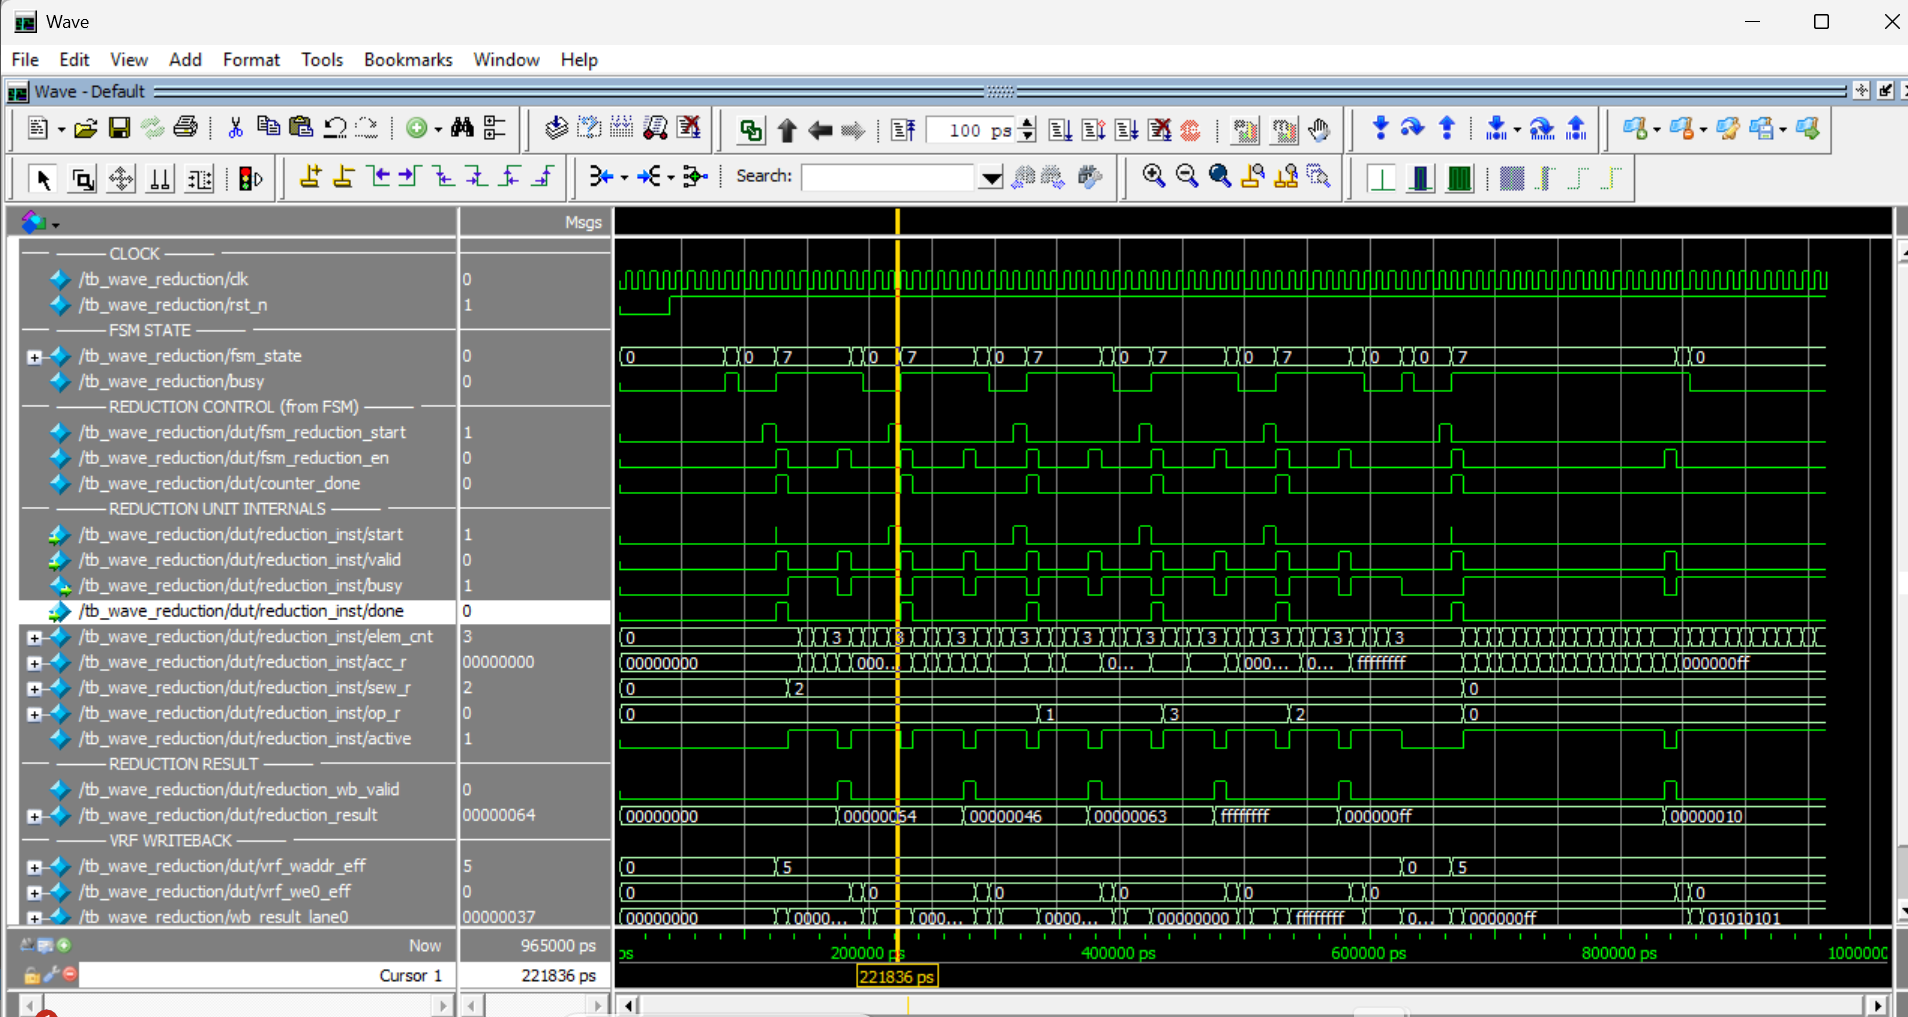
\includegraphics[width=\textwidth]{../image/reduction_sim.png}
  \caption{ModelSim waveform of the reduction unit executing \texttt{vredsum.vs}:
           FSM state transitions, \texttt{busy}/\texttt{done} handshake,
           per-element \texttt{acc\_r} accumulation, and VRF writeback.}
  \label{fig:reduction_wave}
\end{figure}

\subsection{Vector Load/Store Unit}
\label{subsec:vlsu}

The \gls{vlsu} implements unit-stride VLE8.v, VLE16.v, VLE32.v (load) and VSE8.v,
VSE16.v, VSE32.v (store) as defined in the RVV specification \cite{rvv-spec-1-0}.
The module is decoupled from the OP-V pipeline: it operates in parallel with the \gls{fsm},
using the secondary port of \texttt{dmem\_sync} (port~B), while the \gls{fsm} may
execute arithmetic instructions on different registers concurrently.

\subsubsection{Address Calculation}

The VLSU issues word-aligned memory requests. The byte address of the $i$-th 32-bit
word is:

\begin{equation}
\mathit{byte\_addr}[i] = \mathit{rs1\_data} + i \times 4
\label{eq:vlsu_addr}
\end{equation}

where \texttt{rs1\_data} is the base address from the scalar register file, passed at
dispatch time. The VLSU internally increments a word counter (\texttt{word\_ctr\_r})
and multiplies by four using a left-shift (\texttt{\{req\_ctr[29:0], 2'b00\}}), which
synthesises to a simple wire connection rather than an arithmetic unit.

\subsubsection{Load Path}

The VLSU uses a pipelined prefetch strategy to keep the synchronous memory bus busy
on every cycle. When a VLE instruction is dispatched:

\begin{enumerate}
  \item In the same cycle (ST\_IDLE, \texttt{vls\_valid = 1}), a prefetch request for
    word~0 is issued to \texttt{dmem\_sync}. Since the memory has one-cycle registered
    output, the data for word~0 arrives on the first ST\_LOAD cycle.
  \item In ST\_LOAD, the request for word~$n+1$ is issued while the data for word~$n$
    is captured (one cycle earlier request). The word counter advances each cycle that
    \texttt{mem\_ready} is asserted.
  \item Every four consecutive words fill one lane group (\texttt{load\_buf\_r[0:3]}).
    When a group is complete (lane index 3 reached, or last word), a \gls{vrf} write
    is triggered (\texttt{vrf\_we = 1}) for all four lanes simultaneously.
\end{enumerate}

The number of required words is computed at issue time using ceiling-division formulas
(\texttt{num\_words\_comb}) to account for partial trailing words when \texttt{vl}
is not a multiple of the elements-per-word count.

\subsubsection{Store Path}

For a VSE instruction, the \gls{vlsu} reads the source register from the \gls{vrf}
via port~vs2. The wrapper multiplexes the vs2 address input of all four \gls{vrf}
banks to \texttt{vlsu\_vrf\_raddr} during a store operation, overriding the normal
arithmetic address. One word per cycle is written to \texttt{dmem\_sync}:

\begin{equation}
\mathit{store\_word} = \mathit{vrf\_lane[lane\_idx]}
\end{equation}

where \texttt{lane\_idx = word\_ctr\_r[1:0]} selects among the four 32-bit lanes of
the current register.

\subsubsection{Masked Store and Tail Suppression}

For masked store instructions (\texttt{vm = 0}), the byte-enable signals are derived
from the v0 mask register. For each 32-bit word $w$, the byte enable is computed
from the v0 bits corresponding to the elements contained in that word:

\begin{description}
  \item[SEW=8 (4 elements/word):] \texttt{mask\_be[j] = v0\_flat[\{word\_ctr[4:0], j[1:0]\}]}
    for $j \in \{0,1,2,3\}$.
  \item[SEW=16 (2 elements/word):] \texttt{mask\_be[1:0] = \{2\{v0[2k]\}\}},
    \texttt{mask\_be[3:2] = \{2\{v0[2k+1]\}\}} where $k = \mathit{word\_ctr}$.
  \item[SEW=32 (1 element/word):] \texttt{mask\_be = v0[word\_ctr] ? 4'b1111 : 4'b0000}.
\end{description}

An additional \texttt{last\_word\_be} term suppresses tail bytes in the final word of
a transfer when \texttt{vl} is not aligned to a word boundary. For SEW=8:

\begin{equation}
\mathit{last\_word\_be} = \begin{cases}
  4\text{'b0001} & \text{if } \mathit{vl} \bmod 4 = 1 \\
  4\text{'b0011} & \text{if } \mathit{vl} \bmod 4 = 2 \\
  4\text{'b0111} & \text{if } \mathit{vl} \bmod 4 = 3 \\
  4\text{'b1111} & \text{if } \mathit{vl} \bmod 4 = 0 \;(\text{full word})
\end{cases}
\label{eq:last_word_be}
\end{equation}

The effective byte enable for a store word is:

\begin{equation}
\mathit{mem\_be} = (\mathit{last\_word} \;?\; \mathit{last\_word\_be\_r} : 4\text{'b1111})
                   \;\mathbin{\&}\; \mathit{mask\_be}
\label{eq:mem_be}
\end{equation}

This ensures that neither tail elements nor masked elements are written to memory.

\begin{figure}[H]
  \centering
  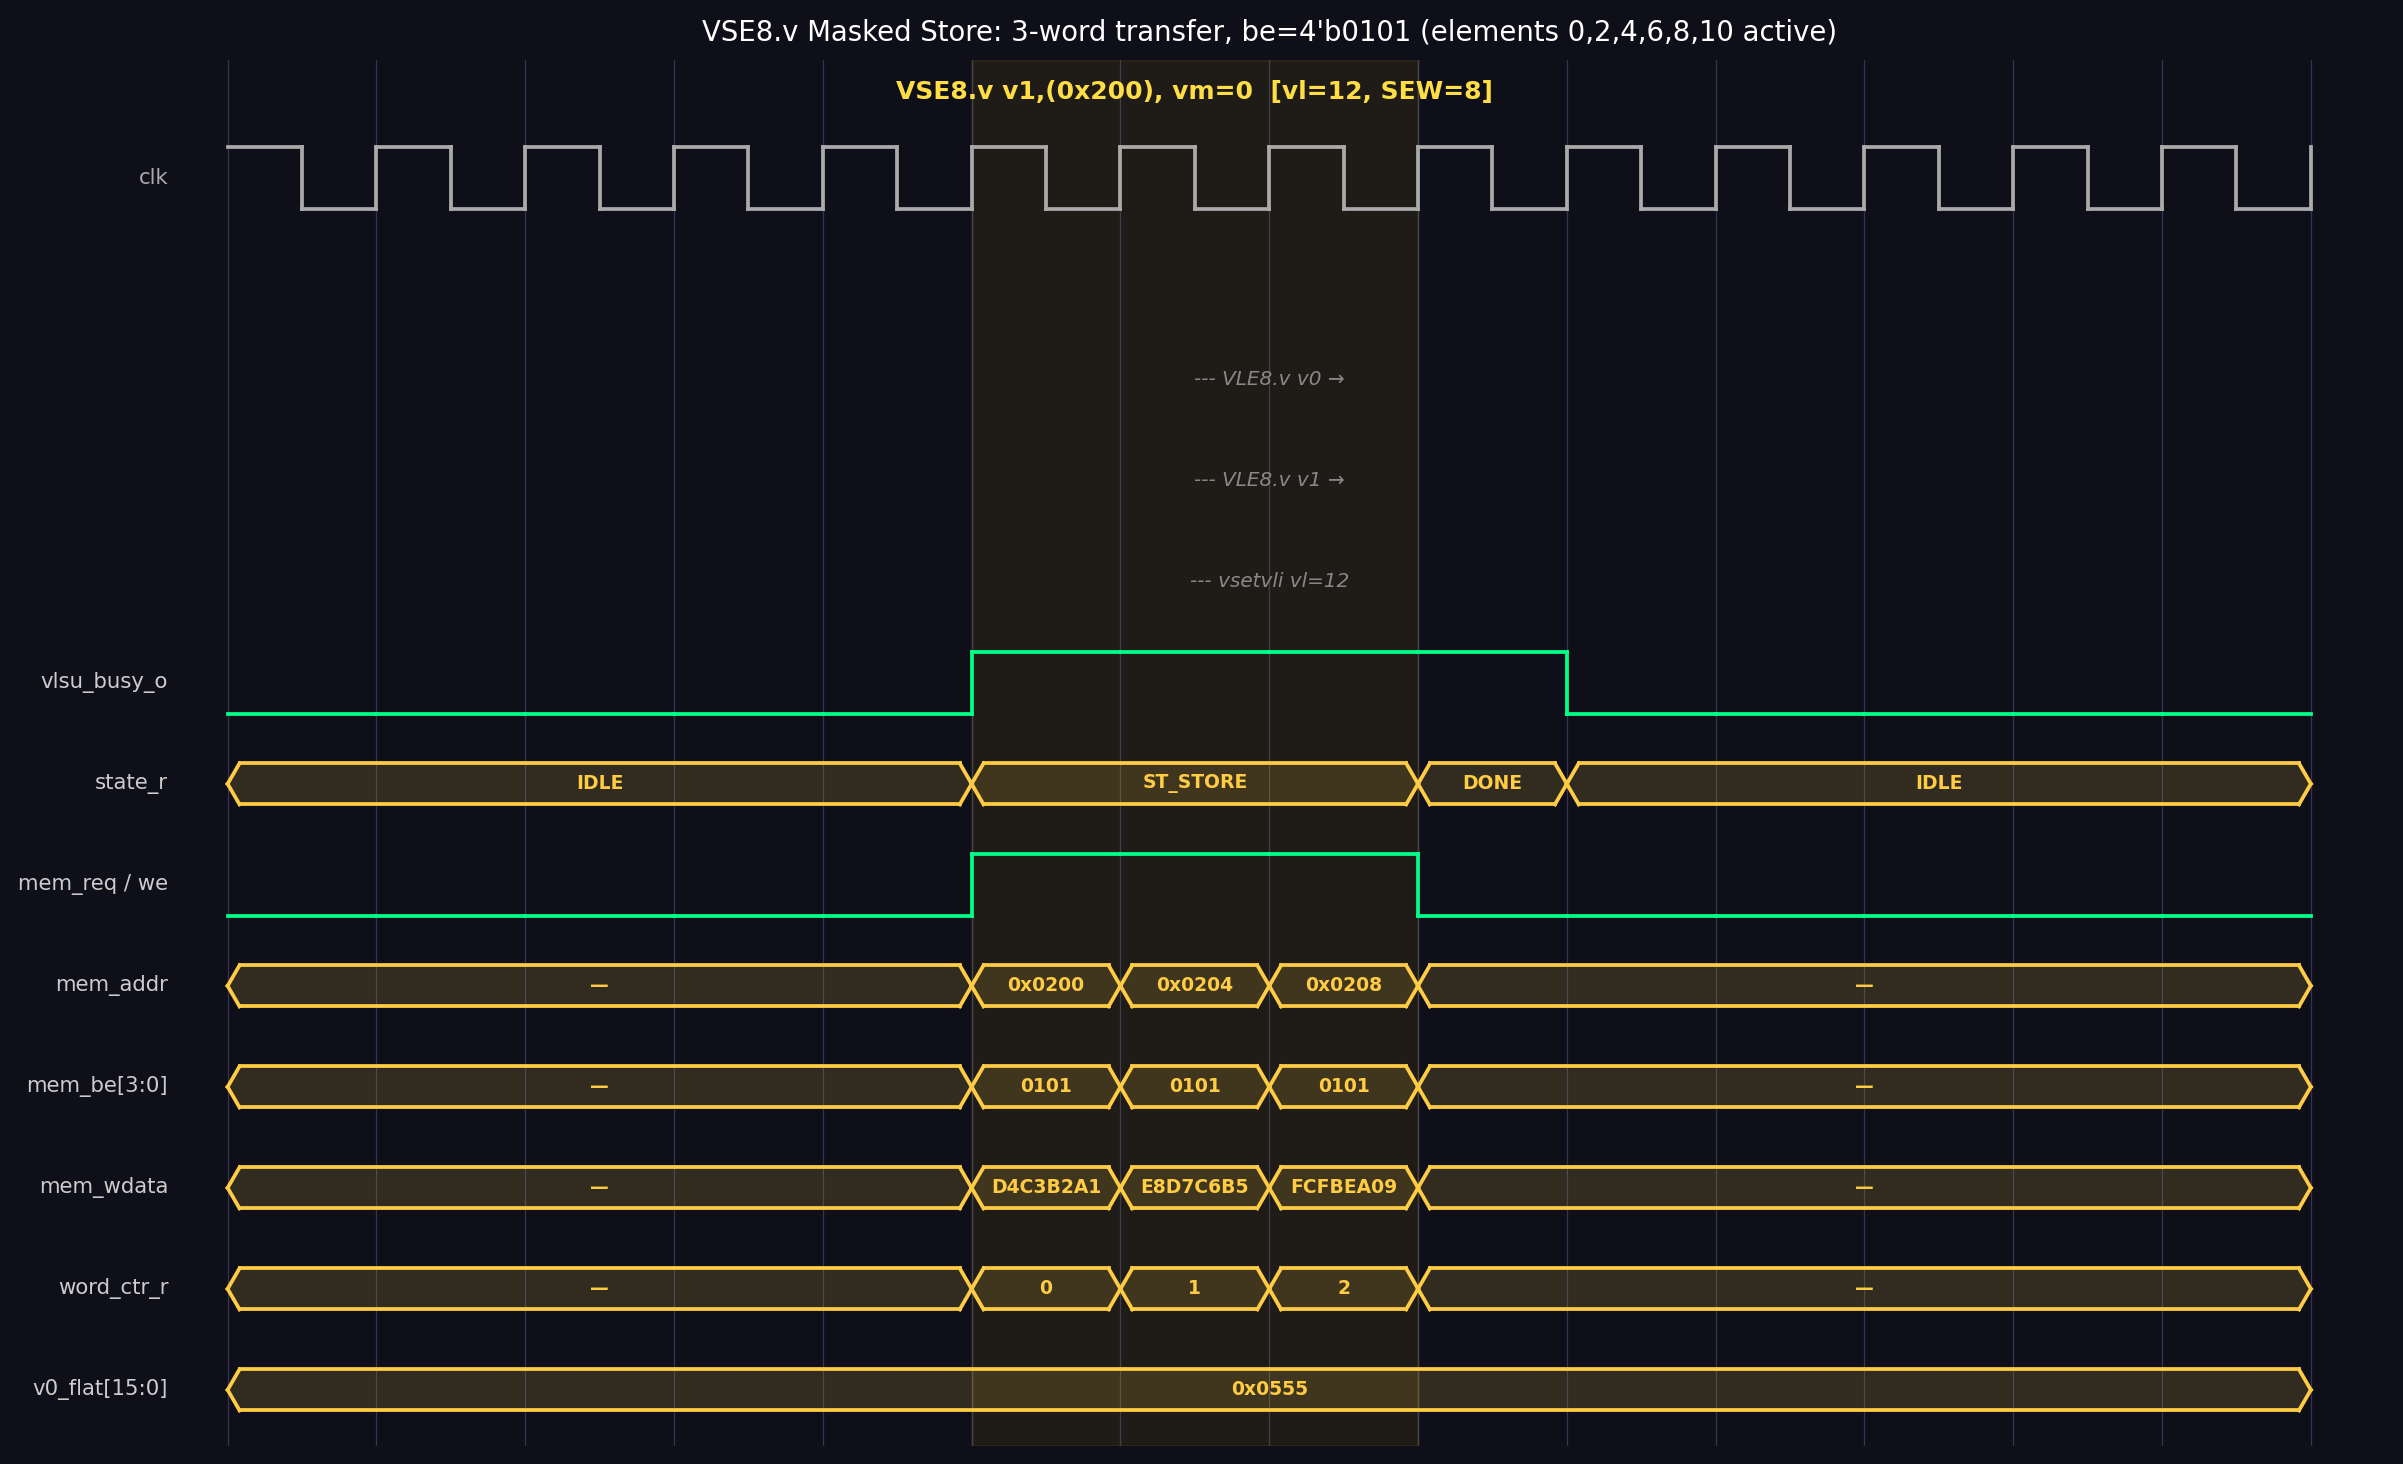
\includegraphics[width=\textwidth]{../image/vlsu_masked_store_wave.png}
  \caption{\texttt{VSE8.v} masked store timing: \texttt{vl}=12, SEW=8, \texttt{vm}=0.
           Three consecutive DMEM words issued (\texttt{0x0200}--\texttt{0x0208}).
           \texttt{mem\_be}=\texttt{4'b0101} every word (elements 0,2,4,6,8,10 active;
           odd elements masked). \texttt{v0\_flat[15:0]}=\texttt{0x0555} holds
           the packed mask register. \texttt{vlsu\_busy\_o} is asserted for the
           full ST\_STORE window.}
  \label{fig:vlsu_masked_wave}
\end{figure}

\subsubsection{Hazard Avoidance}

The wrapper implements a 32-bit scoreboard (\texttt{vrf\_busy\_r}) to prevent
load-use hazards between the \gls{vlsu} and the OP-V pipeline:

\begin{enumerate}
  \item When a VLE instruction is dispatched, \texttt{vrf\_busy\_r[vd\_addr]} is set.
  \item The OP-V \gls{fsm} is held in ST\_IDLE (\texttt{raw\_stall}) if the head-of-FIFO
    instruction reads a register marked as busy.
  \item When the VLSU completes the load (writes the final \gls{vrf} word), the
    busy bit is cleared.
\end{enumerate}

A WAW guard prevents a load from firing while the OP-V \gls{fsm} is writing the same
destination register (\texttt{load\_waw\_stall}). A WAR guard prevents a store from
firing while any instruction in the OP-V pipeline could still be reading the source
register (\texttt{is\_store\_stall = fifo\_or\_fsm\_busy \&\& is\_vls\_store\_raw}).

%% =============================================================================
\section{UART Controller}
\label{sec:uart}
%% =============================================================================

The \gls{uart} peripheral implements 8N1 framing at a configurable baud rate. It is
accessed exclusively by the scalar core via memory-mapped I/O at base address
\texttt{0xFF00\_0000}. The controller is instantiated as a TL-UL slave; the
top-level module constructs TL-UL A-channel and D-channel bundles inline from the
scalar DMEM port signals when a \gls{uart} address is detected.

\subsection{8N1 Framing}

Each transmitted or received frame consists of:
\begin{enumerate}
  \item One start bit (logic 0).
  \item Eight data bits (LSB first).
  \item One stop bit (logic 1).
\end{enumerate}

The total frame length is 10 bit-periods. The receiver uses 16$\times$ oversampling: the
baud clock runs at $\mathit{CLK\_FREQ} / \mathit{BAUD\_RATE}$ cycles per bit, and the
sample point is taken at the 8th oversample count (mid-bit). This tolerates a
$\pm$4/16~=~$\pm$25\% baud-rate error before a mis-sample occurs, well in excess of the
typical crystal-oscillator accuracy of $\pm$100~ppm.

\subsection{MMIO Register Map}

\begin{table}[H]
\centering
\caption{UART memory-mapped register map (base address \texttt{0xFF00\_0000})}
\label{tab:uart_regs}
\begin{tabular}{cllp{6.5cm}}
\toprule
\textbf{Offset} & \textbf{Name} & \textbf{Access} & \textbf{Description} \\
\midrule
\texttt{+0x00} & --- & --- & Reserved (control; not used in current firmware) \\
\texttt{+0x04} & \texttt{STAT}  & R & Status register.
  Bit~[1] = \texttt{RX\_VALID} (1 when RX FIFO non-empty);
  Bit~[0] = \texttt{TX\_BUSY} (1 when TX shift-register active) \\
\texttt{+0x08} & \texttt{TXDAT} & W & Write byte to transmit.
  Writing enqueues one byte into the TX FIFO.
  Ignored if TX FIFO is full. \\
\texttt{+0x0C} & \texttt{RXDAT} & R & Read byte from RX FIFO.
  Returns the oldest received byte and dequeues it.
  Returns \texttt{0x00} if RX FIFO is empty. \\
\bottomrule
\end{tabular}
\end{table}

\subsection{Integration and TL-UL Interface}

The top-level module translates scalar DMEM transactions to TL-UL without a bus
arbiter. The inline address decoder (\texttt{uart\_sel = addr[31:8] == 24'hFF0000})
performs the steering combinatorially. Write transactions set
\texttt{tl\_a.opcode = TL\_A\_PUT\_PARTIAL} with \texttt{tl\_a.mask = s\_dmem\_be};
read transactions set \texttt{tl\_a.opcode = TL\_A\_GET}.

Because \texttt{dmem\_sync} has a one-cycle read latency, the UART response is
registered for one cycle to align with the expected timing: a read issued in cycle $T$
produces data at the scalar WB stage in cycle $T+1$. The registered response is
selected over the DMEM read data via \texttt{uart\_rd\_pending\_r}.

\subsection{FIFO Depth and Overflow Behaviour}

Both the transmit and receive FIFOs have a depth of 8 bytes. The TX FIFO prevents
CPU polling loops from becoming necessary for short bursts: the scalar core can write
up to 8 bytes without waiting for transmission to complete. TX overflow is handled
silently by the FIFO (new write is dropped when full); firmware is expected to poll
\texttt{STAT.TX\_BUSY} before writing.

The RX FIFO prevents character loss during firmware processing delays. At 115\,200~baud,
one character takes approximately 87~$\mu$s; the 8-byte FIFO provides approximately
700~$\mu$s of tolerance before overflow.

%% =============================================================================
\section{Memory Subsystem}
\label{sec:memory}
%% =============================================================================

The system uses a Harvard-style architecture with separate instruction and data address
spaces. This simplifies the timing analysis on the instruction path (no competition
with data traffic) and makes it impossible for self-modifying code to execute, a
constraint that is acceptable for an ASIC accelerator with fixed firmware.

\subsection{Instruction Memory (\texttt{imem\_sync})}
\label{subsec:imem}

\texttt{imem\_sync} is parameterised by \texttt{DEPTH} (default 2048 words, 8~KB) and
\texttt{HEX\_FILE} (default \texttt{"imem.hex"}). At elaboration time, the memory
array is initialised via \texttt{\$readmemh}, which is supported by all major synthesis
flows as a memory-initialisation mechanism.

The output is registered: the instruction word appears at \texttt{instr} one cycle after
the program counter is presented. This matches the synchronous SRAM model used in ASIC
implementations and avoids a long combinational path from PC to decode logic.

Two override conditions modify the registered output:
\begin{itemize}
  \item \textbf{flush}: On a branch-taken or jump (\texttt{pc\_sel = 1}), the output
    register is loaded with the NOP encoding (\texttt{32'h0000\_0013}) to prevent the
    incorrectly-fetched instruction from reaching the decode stage.
  \item \textbf{stall}: When any stall condition (\texttt{stall\_ld} or \texttt{vpu\_stall})
    is active, the clock enable on the output register is held low, preserving the
    current instruction word so it can be re-decoded.
\end{itemize}

\begin{lstlisting}[language=SV,
  caption={\texttt{imem\_sync}: synchronous registered output with flush and stall},
  label={lst:imem_sync}]
always_ff @(posedge clk) begin
    if (reset || flush)  instr <= NOP;      // 32'h00000013
    else if (!stall)     instr <= mem[pc[AW+1:2]];
end
\end{lstlisting}

The address index \texttt{pc[AW+1:2]} discards the two LSBs (byte offset) and limits
the upper bound to $\log_2(\mathit{DEPTH})$ bits, matching a byte-addressed word-aligned
memory array.

\subsection{Data Memory (\texttt{dmem\_sync})}
\label{subsec:dmem}

\texttt{dmem\_sync} is a 64~KB (16\,384-word) dual-port synchronous SRAM with a third
video read port (unused in the simulation top). Port~A is the scalar core's load/store
port; port~B is the exclusive property of the \gls{vlsu}. Both ports use 32-bit words
with byte-enable granularity.

\textbf{Port priority.} When both ports attempt to access the same word-aligned address
in the same cycle, port~A (scalar) takes priority. This design decision avoids
write-after-read conflicts in the typical scalar-store / vector-load sequence where the
scalar core writes a base address and the \gls{vlsu} immediately reads a nearby location.

\textbf{Synchronous read latency.} Both ports register their read data, delivering the
result one cycle after the read request. The scalar core's WB stage is designed to
accept this one-cycle latency. The \gls{vlsu} accounts for this latency through its
prefetch strategy described in Section~\ref{subsec:vlsu}.

\subsection{Memory Address Map}
\label{subsec:memmap}

\begin{table}[H]
\centering
\caption{System memory address map}
\label{tab:memmap}
\begin{tabular}{llll}
\toprule
\textbf{Start Address} & \textbf{End Address} & \textbf{Size} & \textbf{Contents / Notes} \\
\midrule
\texttt{0x0000\_0000} & \texttt{0x0000\_1FFF} & 8~KB   & IMEM (read-only; Harvard)  \\
\texttt{0x0000\_0000} & \texttt{0x0000\_FFFF} & 64~KB  & DMEM scalar port A        \\
\texttt{0x0000\_0000} & \texttt{0x0000\_FFFF} & 64~KB  & DMEM VLSU port B          \\
\texttt{0x0000\_0000} & \texttt{0x0000\_3FFF} & 16~KB  & Lena channel R (pixel data) \\
\texttt{0x0000\_4000} & \texttt{0x0000\_7FFF} & 16~KB  & Lena channel G \\
\texttt{0x0000\_8000} & \texttt{0x0000\_BFFF} & 16~KB  & Lena channel B \\
\texttt{0x0000\_C000} & \texttt{0x0000\_FFFF} & 16~KB  & Lena luminance Y (output)  \\
\texttt{0x0001\_0000} & \texttt{0x0001\_0FFF} & 4~KB   & IO-mapped peripherals (LEDs, HEX) \\
\texttt{0xFF00\_0000} & \texttt{0xFF00\_000F} & 16~B   & UART registers (STAT, TXDAT, RXDAT) \\
\bottomrule
\end{tabular}
\end{table}

\subsection{Harvard Architecture Tradeoffs}
\label{subsec:harvard_tradeoffs}

The Harvard architecture was chosen for the following reasons:

\begin{description}
  \item[Timing simplicity.] Instruction fetch and data access never compete for the
    same memory port. The PC-to-instruction critical path is bounded by the IMEM
    registered output, which is simple to time-analyse.
  \item[Security.] The scalar core cannot write to IMEM. This makes it impossible
    for buggy vector programs to corrupt the instruction stream.
  \item[Synthesis feasibility.] Two independent memory arrays are easier to place and
    route than a unified shared memory requiring a crossbar arbiter.
\end{description}

The main drawback is the inability to load code at runtime without an external JTAG
or SPI programming interface. For a fixed-function accelerator, this is not a
limitation; firmware is compiled and loaded at tapeout time via the \texttt{imem.hex}
initialisation file.

%% =============================================================================
\section{Chapter Summary}
\label{sec:hw_summary}
%% =============================================================================

\begin{table}[H]
\centering
\caption{RTL module summary}
\label{tab:module_summary}
\begin{tabular}{p{4.5cm}p{4.5cm}p{3.5cm}r}
\toprule
\textbf{Module} & \textbf{Function} & \textbf{Key Parameters} & \textbf{Approx. RTL Lines} \\
\midrule
\texttt{riscv\_vpu\_top\_v4}      & System integration, address decode, reset inversion
                                   & CLK\_FREQ, BAUD\_RATE  & 246  \\
\texttt{pipelined\_vpu}           & 5-stage RISC-V pipeline (rv32im\_zicsr)
                                   & ---                    & 698  \\
\texttt{vproc\_system\_wrapper}   & VPU subsystem top, VLSU–FSM–lane integration
                                   & NUM\_REGS, CTRL\_WIDTH & 821  \\
\texttt{vproc\_vdecoder}          & Combinational 32-bit $\to$ 49-bit ctrl\_bus decoder
                                   & CTRL\_WIDTH            & $\sim$200 \\
\texttt{vproc\_fifo}              & Circular instruction queue, depth 8
                                   & DEPTH, CTRL\_WIDTH     & 82   \\
\texttt{vproc\_fsm}               & 9-state execution sequencer
                                   & ---                    & 216  \\
\texttt{vproc\_vregfile}          & 32$\times$8b register bank (4$\times$ instantiated)
                                   & NUM\_REGS              & 73   \\
\texttt{vproc\_vrf\_addr\_gen}    & LMUL-aware source/dest address counters
                                   & ADDR\_WIDTH            & 51   \\
\texttt{vproc\_processor\_lane}   & Execution lane, funct6 result mux, mask apply
                                   & ---                    & 246  \\
\texttt{vproc\_adder}             & SEW-aware add/sub/adc/sbc with widening
                                   & ---                    & 163  \\
\texttt{vproc\_mul}               & SEW-aware multiply (low/high/widening)
                                   & ---                    & $\sim$120 \\
\texttt{vproc\_shifter}           & Logical/arithmetic shift, SEW amount masking
                                   & ---                    & $\sim$80  \\
\texttt{vproc\_logic}             & Bitwise AND/OR/XOR
                                   & ---                    & $\sim$30  \\
\texttt{vproc\_compare}           & Element-wise compare, 4-bit result
                                   & ---                    & $\sim$80  \\
\texttt{vproc\_minmax}            & Signed/unsigned per-element min/max
                                   & ---                    & $\sim$80  \\
\texttt{vproc\_reduction}         & Serial accumulator for vred* instructions
                                   & ---                    & 135  \\
\texttt{vproc\_vec\_lsu}          & Unit-stride VLE/VSE with masked stores
                                   & VLEN, REG\_AWIDTH      & 381  \\
\texttt{vproc\_cycle\_counter}    & vl-aware execution cycle and mask counter
                                   & ---                    & $\sim$100 \\
\texttt{vproc\_mask\_enable}      & Per-lane mask-bit extraction from v0 flat
                                   & ---                    & $\sim$80  \\
\texttt{vproc\_mask\_write\_buffer} & Bit accumulation buffer for mask results
                                   & ---                    & $\sim$70  \\
\texttt{vproc\_merge\_unit}       & VMERGE / VMV element selection
                                   & ---                    & $\sim$60  \\
\texttt{vproc\_vcsr}              & vl / vtype / vlenb CSR storage
                                   & ---                    & $\sim$60  \\
\texttt{vproc\_cfg\_encoder}      & vl = min(avl, vlmax) computation from vtype
                                   & ---                    & $\sim$60  \\
\texttt{imem\_sync}               & 8~KB synchronous instruction memory
                                   & DEPTH                  & 28   \\
\texttt{dmem\_sync}               & 64~KB dual-port synchronous data memory
                                   & DEPTH                  & $\sim$100 \\
\texttt{uart}                     & 8N1 UART with TL-UL slave interface
                                   & CLK\_FREQ, BAUD\_RATE  & $\sim$300 \\
\bottomrule
\multicolumn{3}{l}{\textbf{Total (estimated)}} & $\mathbf{\sim}$\textbf{4{,}700} \\
\bottomrule
\end{tabular}
\end{table}

This chapter has presented the complete hardware design of the RISC-V VPU system.
The five-stage scalar pipeline provides a standard in-order RV32IM execution engine
with full forwarding and load-use stall detection. The VPU subsystem is decoupled from
the scalar pipeline via a depth-8 instruction FIFO; the nine-state \gls{fsm} sequences
all instruction categories including multi-cycle widening, mask accumulation, and the
serial reduction protocol. The \gls{vrf} is organised as four parallel 8-bit banks,
enabling byte-granularity write masking and efficient clock-gating inference. The
vector \gls{vlsu} handles unit-stride loads and stores with a pipelined prefetch
strategy, a scoreboard for RAW/WAW/WAR hazard prevention, and a precise tail-byte
suppression mechanism. The \gls{uart} and dual-port memory subsystem complete the
integration, providing both host communication and the data-bandwidth required for
image-processing workloads.
